\begin{singlespace}
    \chapter{\textbf{The relative cost of resource use for photosynthesis drives variance in leaf nitrogen content across a climate and soil resource availability gradient}}
\end{singlespace}

\section{Introduction}
\noindent Terrestrial biosphere models, which comprise the land surface component of Earth system models, are sensitive to the formulation of photosynthetic processes \shortcite{KnorrHeimann2001,Ziehn2011,Booth2012,Walker2021}. This is because photosynthesis is the largest carbon flux between the atmosphere and terrestrial biosphere \shortcite{IPCC2021}, and is constrained by ecosystem carbon and nutrient cycles \shortcite{Hungate2003,LeBauer2008,Fay2015}. Many terrestrial biosphere models parameterize photosynthetic capacity through plant functional group specific empirical linear relationships between area-based leaf nitrogen content ($N_\mathrm{area}$) and the maximum carboxylation rate of Ribulose-1,5-bisphosphate carboxylase/oxygenase ($V_\mathrm{cmax}$) \shortcite{Kattge2009,Rogers2014,Rogers2017a}. Models are beginning to include connected carbon-nitrogen cycles \shortcite{Wieder2015_NPP,Shi2016,Davies-Barnard2020,Braghiere2022}, which allows models to predict leaf photosynthesis directly through changes in $N_\mathrm{area}$ and indirectly through changes in soil nitrogen availability (e.g., LPJ-GUESS, CLM5.0) \shortcite{Smith2014,Lawrence2019}. Despite recent model developments, open questions remain regarding the generality of ecological relationships between soil nitrogen availability, leaf nitrogen content, and leaf photosynthesis across edaphic and climatic gradients.

Empirical support for positive relationships between soil nitrogen availability and $N_\mathrm{area}$ is abundant \shortcite{Firn2019,Liang2020}, and is a result often attributed to the high nitrogen cost of building and maintaining Rubisco \shortcite{Evans1989_photoN,EvansSeemann1989,Onoda2004,Walker2014,Onoda2017,Dong2020}. Such patterns imply that positive relationships between soil nitrogen availability and $N_\mathrm{area}$ should increase net photosynthesis by increasing nutrient allocation to photosynthetic enzyme construction and maintenance. This integrated $N_\mathrm{area}$-photosynthesis response to soil nitrogen availability has been observed both in manipulative experiments and across environmental gradients \shortcite{Field1986,Evans1989_photoN,Walker2014,Li2020}, and is thought to be driven by ecosystem nitrogen limitation, which limits primary productivity globally \shortcite{LeBauer2008,Fay2015}. However, recent studies note variable $N_\mathrm{area}$-photosynthesis relationships across edaphic and climatic gradients \shortcite{Liang2020,Luo2021} and that aboveground growing conditions (e.g., light availability, temperature, vapor pressure deficit) or species identity traits (e.g., photosynthetic pathway, dominant mode of nutrient acquisition) may be more important for explaining variance in $N_\mathrm{area}$ and photosynthetic capacity across environmental gradients \shortcite{Adams2016,Dong2017,Smith2019,Dong2020,Peng2021,Dong2022a,Westerband2023}.

Photosynthetic least-cost theory provides a possible mechanism to explain variance in $N_\mathrm{area}$ across environmental gradients \shortcite{Wright2003,Prentice2014,Paillassa2020,Harrison2021}. The theory predicts that plants acclimate to environments by optimizing photosynthetic assimilation rates at the lowest summed cost of nitrogen and water use \shortcite{Wright2003,Prentice2014}. In a given environment, nitrogen and water use can be substituted for each other to maintain the lowest summed cost of resource use, which alters the cost of acquiring and using nitrogen relative to water, a ratio herein referred to as $\beta$. All else equal, the theory predicts that increasing soil nitrogen availability should decrease $\beta$, resulting in optimal photosynthetic rates achieved with greater $N_\mathrm{area}$ at decreased stomatal conductance and reduced leaf $C_\mathrm{i}$:$C_\mathrm{a}$ \shortcite{Wright2003,Prentice2014,Paillassa2020}. Alternatively, increasing soil moisture should reduce costs of water acquisition and use, therefore increasing $\beta$ \shortcite{Lavergne2020}, stomatal conductance, and leaf $C_\mathrm{i}$:$C_\mathrm{a}$, resulting in optimal photosynthetic rates achieved with decreased $N_\mathrm{area}$. The theory also predicts nitrogen-water use tradeoffs in response to climatic factors, suggesting that the optimal response to increased vapor pressure deficit should be a reduction in stomatal conductance and leaf $C_\mathrm{i}$:$C_\mathrm{a}$ that is counterbalanced by an increase in $N_\mathrm{area}$ to support the greater photosynthetic capacity needed to maintain high assimilation at decreased conductance \shortcite{Grossiord2020,Dong2020,Lopez2021,Westerband2023}.

Leaf nitrogen allocation responses to changing climates or soil resource availability may depend on species' dominant mode of nutrient acquisition. For example, species that form associations with symbiotic nitrogen-fixing bacteria (referred as “N-fixing species” from this point forward) should, in theory, have access to less finite nitrogen supply than species not capable of forming such associations (referred as “non-fixing species” from this point forward), which may result in decreased $\beta$ values in N-fixing species than non-fixing species. This result was previously shown in a greenhouse experiment, where a leguminous species generally had decreased costs of nitrogen acquisition compared to a non-leguminous species, although these differences were generally stronger under increased nitrogen limitation \shortcite{Perkowski2021}. Reduced $\beta$ values could be an explanation for why N-fixing species commonly have greater leaf nitrogen content than non-fixing species \shortcite{Adams2016,Dong2017}.

Similarly, leaf nitrogen allocation patterns across environmental gradients may be dependent on photosynthetic pathway. Reduced leaf $C_\mathrm{i}$:$C_\mathrm{a}$ values in C$_4$ species suggests that C$_4$ species should have reduced $\beta$ values compared to C$_3$ species \shortcite{Scott2022}, a pattern that could be the result of increased costs associated with water acquisition and use or reduced costs of nitrogen acquisition and use relative to C$_3$ species. Theory predicts that this response in C$_4$ species will cause C$_4$ species to have higher leaf nitrogen content on average compared to C$_3$ species, though several studies document decreased leaf nitrogen content in C$_4$ species \shortcite{Schmitt1981,Sage1987_c3c4,Ghannoum2011}. No study to date has directly quantified $\beta$ in C$_4$ species aside from the initial parameterization of $\beta$ in an optimality model for C$_4$ species \shortcite{Scott2022} using a global dataset of leaf $\delta^{13}$C values \shortcite{Cornwell2018}.

While photosynthetic least-cost theory provides a unified framework for understanding integrated effects of climate and soil resource availability on $N_\mathrm{area}$, empirical tests of the theory are sparse. Previous work shows that increasing soil nitrogen availability decreases costs of acquiring nutrients \shortcite{Bae2015,Perkowski2021,Lu2022}, which can induce predictable nutrient-water use tradeoffs expected from the theory across broad environmental gradients \shortcite{Paillassa2020,Querejeta2022,Westerband2023} and in manipulation experiments \shortcite{BialicMurphy2021}. Additionally, increasing vapor pressure deficit has been shown to have a positive effect on $N_\mathrm{area}$, which is commonly associated with reduced leaf $C_\mathrm{i}$:$C_\mathrm{a}$ \shortcite{Dong2017,Dong2020,Firn2019,Lopez2021}.

Despite evidence for patterns expected from photosynthetic least-cost theory, studies have been restricted to exploring these patterns in C$_3$ species and, while variance in $N_\mathrm{area}$ across environmental gradients has been shown to be driven by strong negative relationships with leaf $C_\mathrm{i}$:$C_\mathrm{a}$ \shortcite{Dong2017,Paillassa2020,Westerband2023}, no study has explicitly investigated effects of soil resource availability or species identity on $N_\mathrm{area}$ using $\beta$ as a direct predictor of leaf $C_\mathrm{i}$:$C_\mathrm{a}$. Furthermore, as $N_\mathrm{area}$ can be broken down into structural (leaf mass per area; $M_\mathrm{area}$; g m$^{-2}$) and metabolic (mass-based leaf nitrogen content; $N_\mathrm{mass}$; gN g$^{-1}$) components \shortcite{Dong2017}, no study has investigated which component of $N_\mathrm{area}$ drives the hypothesized response of $N_\mathrm{area}$ to leaf $C_\mathrm{i}$:$C_\mathrm{a}$, which limits our ability to assess whether changes in $N_\mathrm{area}$ across environmental gradients are driven by changes in leaf morphology (i.e. $M_\mathrm{area}$), leaf stoichiometry (i.e. $N_\mathrm{mass}$), or both. 

In this study, I measured $N_\mathrm{area}$, $N_\mathrm{mass}$, $M_\mathrm{area}$, leaf $\delta^{13}$C-derived estimates of leaf $C_\mathrm{i}$:$C_\mathrm{a}$, and $\beta$ in 504 individuals spanning 52 species scattered across 24 grassland sites in Texas, USA. The state of Texas contains a diverse climatic gradient, indicated by 2006-2020 mean annual precipitation totals ranging from 204 to 1803 mm and 2006-2020 mean annual temperature ranging from 11.8\textdegree{} to 24.6\textdegree{}C within state boundaries (Fig. \ref{fig:figure4.1}). Variability in soil nitrogen availability and soil moisture was expected across sites, owing to differences in soil texture and aboveground climate that would drive differential rates of water retention and nitrogen transformations to plant-available nitrogen substrate. I leveraged the expected climatic and soil resource variability across sites to test the following hypotheses:

\begin{enumerate}
    \item Soil nitrogen availability will decrease $\beta$ through a reduction in costs of nitrogen acquisition and use, while soil moisture will increase $\beta$ through a reduction in costs of water acquisition and use. Following previous results, I expected that N-fixing species and C$_4$ species would each have reduced $\beta$ values.
    
    \item Leaf $C_\mathrm{i}$:$C_\mathrm{a}$ will be positively related to $\beta$, a pattern that will result in a negative indirect effect of increasing soil nitrogen availability on leaf $C_\mathrm{i}$:$C_\mathrm{a}$, a positive indirect effect of increasing soil moisture on leaf $C_\mathrm{i}$:$C_\mathrm{a}$, and reduced leaf $C_\mathrm{i}$:$C_\mathrm{a}$ in both N-fixing species and C$_4$ species. I expected that leaf $C_\mathrm{i}$:$C_\mathrm{a}$ would be negatively related to vapor pressure deficit, as increasing atmospheric dryness would cause plants to close stomata to minimize water loss.

    \item $N_\mathrm{area}$ will be negatively related to leaf $C_\mathrm{i}$:$C_\mathrm{a}$. This response will result in an indirect positive and negative effect of increasing soil nitrogen availability and soil moisture, respectively, on $N_\mathrm{area}$, and larger $N_\mathrm{area}$ values in N-fixing species. While theory predicts that reduced $\beta$ values in C$_4$ species should yield larger $N_\mathrm{area}$ in C$_4$ species, I expected that C$_4$ species would have decreased $N_\mathrm{area}$ than $C_3$ species due to greater nitrogen use efficiency in C$_4$ species. Additionally, I expected vapor pressure deficit to increase $N_\mathrm{area}$, a pattern that would be directly mediated through the reduction in leaf $C_\mathrm{i}$:$C_\mathrm{a}$ with increasing vapor pressure deficit.
\end{enumerate}

\section{Methods}
\subsection{\textit{Site descriptions and sampling methodology}}
\noindent Leaf and soil samples were collected from 24 open canopy grassland sites scattered across central and eastern Texas in summer 2020 and summer 2021 (Fig. \ref{fig:figure4.1}). Twelve sites were visited between June and July 2020 and 14 sites (11 unique from 2020) were visited between May and June 2021 (Table \ref{tab:table4.1}). Sites were chosen to maximize precipitation and edaphic variability across sites (Table \ref{tab:table4.1}). No site with personally communicated or anecdotal evidence of grazing or disturbance (e.g., mowing, feral hog activity, etc.) was used. Leaf material was collected from three individuals each of the five most abundant species at random locations at each site, only  selecting species that were broadly classified as graminoid or forb/herb growth habits per the USDA PLANTS database \shortcite{USDANRCS2022}. All collected leaves were fully expanded with no visible herbivory or other external damage and also free from shading by nearby shrubs or trees. Five soil samples were collected from 0-15 cm below the soil surface at each site near the leaf collection sample locations. Soil samples were mixed together by hand to create one composite soil sample per site.

\subsection{\textit{Leaf trait measurements}}
\noindent Images of each leaf were taken immediately following each site visit using a flat-bed scanner. Fresh leaf area was determined from each image using the `LeafArea' R package \shortcite{Katabuchi2015}, which automates leaf area calculations using ImageJ software \shortcite{Schneider2012}. Each leaf was dried at 65\textdegree{}C for at least 48 hours to a constant mass, weighed, and manually ground in a mortar and pestle until homogenized. Leaf mass per area ($M_\mathrm{area}$; g m$^{-2}$) was calculated as the ratio of dry leaf biomass to fresh leaf area. Subsamples of dried and homogenized leaf tissue were used to measure leaf nitrogen content ($N_\mathrm{mass}$; gN g$^{-1}$) through elemental combustion analysis (Costech-4010, Costech Instruments, Valencia, CA). Leaf nitrogen content per unit leaf area ($N_\mathrm{area}$; gN m$^{-2}$) was calculated as the product of $N_\mathrm{mass}$ and $M_\mathrm{area}$.
    
Subsamples of dried and homogenized leaf tissue were sent to the University of California-Davis Stable Isotope Facility to determine leaf $\delta^{13}$C. Leaf $\delta^{13}$C values were determined using an elemental analyzer (PDZ Europa ANCA-GSL; Sercon Ltd., Chestshire, UK) interfaced to an isotope ratio mass spectrometer (PDZ Europa 20-20 Isotope Ratio Mass Spectrometer, Sercon Ltd., Chestshire, UK). I used leaf $\delta^{13}$C values (‰; relative to Vienna Pee Dee Belemnite international reference standard) to estimate the ratio of intercellular ($C_\mathrm{i}$) to extracellular ($C_\mathrm{a}$) CO$_2$ ratio (leaf $C_\mathrm{i}$:$C_\mathrm{a}$; unitless) following the approach of \shortciteN{Farquhar1989} described in \shortciteN{Cernusak2013}. Specifically, I derived leaf $C_\mathrm{i}$:$C_\mathrm{a}$ as:

\begin{equation} 
    \label{eq_4.1}
    C_i:C_a = \frac{\Delta^{13}C - a}{b - a}
\end{equation}
    
\noindent where $\Delta^{13}$C represents the relative difference between leaf $\delta^{13}$C (‰) and air $\delta^{13}$C (‰), calculated as:

\begin{equation}
    \label{eq_4.2}
    \Delta^{13}C = \frac{\delta^{13}C_{air} - \delta^{13}C_{leaf}}{1 + \delta^{13}C_{leaf}}
\end{equation}

\noindent $\delta^{13}\mathrm{C_{air}}$ was assumed to be -8‰ \shortcite{Keeling1979,Farquhar1989}. The parameter \textit{a} represents the fractionation between $^{12}$C and $^{13}$C due to diffusion in air, assumed to be 4.4‰, while \textit{b} represents the fractionation caused by Rubisco carboxylation, assumed to be 27‰ \shortcite{Farquhar1989}. For C$_4$ species, \textit{b} in Eqn. \ref{eq_4.1} was set to 6.3‰, and was derived from:

\begin{equation}
    \label{eq_4.4}
    b = c + (d \cdot \phi)
\end{equation}
    
\noindent Where \textit{c} was set to -5.7‰ and \textit{d} was set to 30‰ \shortcite{Farquhar1989}. $\phi$, which is the bundle sheath leakiness term, was set to 0.4. All leaf $C_\mathrm{i}$:$C_\mathrm{a}$ values less than 0.1 and greater than 0.95 were assumed to be incorrect and removed from the analysis.
    
I derived the unit cost of resource use ($\beta$) using leaf $C_\mathrm{i}$:$C_\mathrm{a}$ and site climate data using equations first described in \shortciteN{Prentice2014} and simplified in \shortciteN{Lavergne2020}:

\begin{equation}
    \label{eq_4.5}
    \beta = 1.6\eta^{*} VPD \frac{\chi - (\frac{\Gamma^*}{C_{a}})^{2}}{(1 - \chi)^{2}(K_{m} + \Gamma^{*})}
\end{equation}
    
\noindent where $\eta^{*}$ is the viscosity of water relative to 25\textdegree{}C, calculated using elevation and mean air temperature of the seven days leading up to each site visit following equations in \shortciteN{Huber2009}. VPD (Pa) was set to the mean vapor pressure deficit of the seven days leading up to each site visit, $C_\mathrm{a}$ represents atmospheric CO$_2$ concentration, arbitrarily set to 420 $\mathrm{\mu mol\ mol^{-1}}$ CO$_2$. $C_\mathrm{a}$ was converted to partial pressure (Pa) and corrected by site elevation. $K_\mathrm{m}$ (Pa) is the Michaelis-Menten coefficient for Rubisco affinity to CO$_2$ and O$_2$, calculated as:
    
\begin{equation} \label{eq_4.6}
    K_{m} = K_{c} \cdot \left ( 1 + \frac{O_i}{K_o} \right )
\end{equation}

\noindent where $K_\mathrm{c}$ (Pa) and $K_\mathrm{o}$ (Pa) are the Michaelis-Menten coefficients for Rubisco affinity to CO$_2$ and O$_2$, respectively, and $O_\mathrm{i}$  is the intercellular O$_2$ concentration. $\Gamma^{*}$ (Pa) is the CO$_2$ compensation point in the absence of dark respiration. $K_\mathrm{c}$, $K_\mathrm{o}$, and $\Gamma^{*}$ were determined using equations described in \shortciteN{Medlyn2002} and derived in \shortciteN{Bernacchi2001}, invoking an elevation correction for atmospheric pressure as explained in \shortciteN{Stocker2020}.
\clearpage

\newpage
\begin{table}
    \centering
    \caption[Site locality information, sampling year, 2006-2020 mean annual precipitation, mean annual temperature, and water holding capacity]{Site locality information, sampling year, 2006-2020 mean annual precipitation (MAP; mm), mean annual temperature (MAT; \textdegree{}C), and water holding capacity (WHC; mm)$^*$}
    \resizebox{\columnwidth}{!}{
        \begin{tabular}{p{5cm}p{3cm}p{3cm}p{3cm}p{3cm}p{3cm}p{3cm}}
            \hline
            \multicolumn{1}{l}{Site} 
            & \multicolumn{1}{r}{Latitude} 
            & \multicolumn{1}{r}{Longitude} 
            & \multicolumn{1}{r}{Sampling year}
            & \multicolumn{1}{r}{MAP}  
            & \multicolumn{1}{r}{MAT} 
            & \multicolumn{1}{r}{WHC} 
            \\
            \hline 

            \multicolumn{1}{l}{Edwards\_2019\_17} 
            & \multicolumn{1}{r}{29.95}
            & \multicolumn{1}{r}{-100.36}
            & \multicolumn{1}{r}{2020}
            & \multicolumn{1}{r}{563.5}
            & \multicolumn{1}{r}{19.0}
            & \multicolumn{1}{r}{224.7}
            \\

            \multicolumn{1}{l}{Uvalde\_2020\_02} 
            & \multicolumn{1}{r}{29.59}
            & \multicolumn{1}{r}{-100.09}
            & \multicolumn{1}{r}{2020, 2021}
            & \multicolumn{1}{r}{648.5}
            & \multicolumn{1}{r}{19.5}
            & \multicolumn{1}{r}{224.7}
            \\

            \multicolumn{1}{l}{Menard\_2020\_01} 
            & \multicolumn{1}{r}{30.91}
            & \multicolumn{1}{r}{-99.59}
            & \multicolumn{1}{r}{2020}
            & \multicolumn{1}{r}{641.9}
            & \multicolumn{1}{r}{18.3}
            & \multicolumn{1}{r}{220.2}
            \\

            \multicolumn{1}{l}{Kerr\_2020\_03} 
            & \multicolumn{1}{r}{30.06}
            & \multicolumn{1}{r}{-99.34}
            & \multicolumn{1}{r}{2021}
            & \multicolumn{1}{r}{672.4}
            & \multicolumn{1}{r}{18.3}
            & \multicolumn{1}{r}{237.5}
            \\

            \multicolumn{1}{l}{Bandera\_2020\_03} 
            & \multicolumn{1}{r}{29.85}
            & \multicolumn{1}{r}{-99.30}
            & \multicolumn{1}{r}{2021}
            & \multicolumn{1}{r}{789.4}
            & \multicolumn{1}{r}{18.8}
            & \multicolumn{1}{r}{235.1}
            \\

            \multicolumn{1}{l}{Sansaba\_2020\_01} 
            & \multicolumn{1}{r}{31.29}
            & \multicolumn{1}{r}{-98.62}
            & \multicolumn{1}{r}{2020}
            & \multicolumn{1}{r}{733.0}
            & \multicolumn{1}{r}{18.8}
            & \multicolumn{1}{r}{234.3}
            \\

            \multicolumn{1}{l}{Comal\_2020\_21} 
            & \multicolumn{1}{r}{29.79}
            & \multicolumn{1}{r}{-98.43}
            & \multicolumn{1}{r}{2020}
            & \multicolumn{1}{r}{878.5}
            & \multicolumn{1}{r}{19.9}
            & \multicolumn{1}{r}{220.7}
            \\

            \multicolumn{1}{l}{Blanco\_2019\_16} 
            & \multicolumn{1}{r}{29.99}
            & \multicolumn{1}{r}{-98.43}
            & \multicolumn{1}{r}{2020}
            & \multicolumn{1}{r}{833.0}
            & \multicolumn{1}{r}{19.2}
            & \multicolumn{1}{r}{222.2}
            \\

            \multicolumn{1}{l}{Bexar\_2019\_13} 
            & \multicolumn{1}{r}{29.24}
            & \multicolumn{1}{r}{-98.43}
            & \multicolumn{1}{r}{2020}
            & \multicolumn{1}{r}{759.3}
            & \multicolumn{1}{r}{21.5}
            & \multicolumn{1}{r}{206.0}
            \\

            \multicolumn{1}{l}{Burnet\_2020\_14} 
            & \multicolumn{1}{r}{30.84}
            & \multicolumn{1}{r}{-98.34}
            & \multicolumn{1}{r}{2021}
            & \multicolumn{1}{r}{763.3}
            & \multicolumn{1}{r}{19.5}
            & \multicolumn{1}{r}{217.8}
            \\

            \multicolumn{1}{l}{Comal\_2020\_19} 
            & \multicolumn{1}{r}{30.01}
            & \multicolumn{1}{r}{-98.32}
            & \multicolumn{1}{r}{2021}
            & \multicolumn{1}{r}{845.0}
            & \multicolumn{1}{r}{19.3}
            & \multicolumn{1}{r}{220.4}
            \\

            \multicolumn{1}{l}{Hays\_2020\_54} 
            & \multicolumn{1}{r}{29.96}
            & \multicolumn{1}{r}{-98.17}
            & \multicolumn{1}{r}{2021}
            & \multicolumn{1}{r}{861.3}
            & \multicolumn{1}{r}{20.0}
            & \multicolumn{1}{r}{225.6}
            \\

            \multicolumn{1}{l}{Burnet\_2020\_12} 
            & \multicolumn{1}{r}{30.82}
            & \multicolumn{1}{r}{-98.06}
            & \multicolumn{1}{r}{2021}
            & \multicolumn{1}{r}{815.1}
            & \multicolumn{1}{r}{19.4}
            & \multicolumn{1}{r}{245.3}
            \\
            
            \multicolumn{1}{l}{Williamson\_2019\_09} 
            & \multicolumn{1}{r}{30.71}
            & \multicolumn{1}{r}{-97.86}
            & \multicolumn{1}{r}{2020}
            & \multicolumn{1}{r}{867.7}
            & \multicolumn{1}{r}{19.7}
            & \multicolumn{1}{r}{270.2}
            \\

            \multicolumn{1}{l}{Williamson\_2019\_10} 
            & \multicolumn{1}{r}{30.54}
            & \multicolumn{1}{r}{-97.77}
            & \multicolumn{1}{r}{2020}
            & \multicolumn{1}{r}{819.5}
            & \multicolumn{1}{r}{19.9}
            & \multicolumn{1}{r}{239.8}
            \\

            \multicolumn{1}{l}{Bell\_2021\_08} 
            & \multicolumn{1}{r}{31.06}
            & \multicolumn{1}{r}{-97.55}
            & \multicolumn{1}{r}{2021}
            & \multicolumn{1}{r}{937.3}
            & \multicolumn{1}{r}{19.6}
            & \multicolumn{1}{r}{232.3}
            \\

            \multicolumn{1}{l}{Fayette\_2021\_12} 
            & \multicolumn{1}{r}{29.86}
            & \multicolumn{1}{r}{-97.21}
            & \multicolumn{1}{r}{2021}
            & \multicolumn{1}{r}{985.7}
            & \multicolumn{1}{r}{20.4}
            & \multicolumn{1}{r}{165.6}
            \\

            \multicolumn{1}{l}{Fayette\_2019\_04} 
            & \multicolumn{1}{r}{30.09}
            & \multicolumn{1}{r}{-96.78}
            & \multicolumn{1}{r}{2020}
            & \multicolumn{1}{r}{1017.4}
            & \multicolumn{1}{r}{20.6}
            & \multicolumn{1}{r}{226.9}
            \\

            \multicolumn{1}{l}{Fayette\_2020\_09} 
            & \multicolumn{1}{r}{29.86}
            & \multicolumn{1}{r}{-96.71}
            & \multicolumn{1}{r}{2021}
            & \multicolumn{1}{r}{1002.7}
            & \multicolumn{1}{r}{20.8}
            & \multicolumn{1}{r}{187.6}
            \\

            \multicolumn{1}{l}{Washington\_2020\_08} 
            & \multicolumn{1}{r}{30.28}
            & \multicolumn{1}{r}{-96.41}
            & \multicolumn{1}{r}{2021}
            & \multicolumn{1}{r}{1077.4}
            & \multicolumn{1}{r}{20.4}
            & \multicolumn{1}{r}{203.9}
            \\

            \multicolumn{1}{l}{Austin\_2020\_03} 
            & \multicolumn{1}{r}{29.78}
            & \multicolumn{1}{r}{-96.24}
            & \multicolumn{1}{r}{2021}
            & \multicolumn{1}{r}{1108.7}
            & \multicolumn{1}{r}{20.6}
            & \multicolumn{1}{r}{253.0}
            \\

            \multicolumn{1}{l}{Brazos\_2020\_16} 
            & \multicolumn{1}{r}{30.93}
            & \multicolumn{1}{r}{-96.23}
            & \multicolumn{1}{r}{2021}
            & \multicolumn{1}{r}{1078.0}
            & \multicolumn{1}{r}{20.1}
            & \multicolumn{1}{r}{202.2}
            \\

            \multicolumn{1}{l}{Brazos\_2020\_18} 
            & \multicolumn{1}{r}{30.52}
            & \multicolumn{1}{r}{-96.21}
            & \multicolumn{1}{r}{2020, 2021}
            & \multicolumn{1}{r}{1099.4}
            & \multicolumn{1}{r}{20.4}
            & \multicolumn{1}{r}{233.5}
            \\

            \multicolumn{1}{l}{Harris\_2020\_03} 
            & \multicolumn{1}{r}{29.88}
            & \multicolumn{1}{r}{-95.31}
            & \multicolumn{1}{r}{2020, 2021}
            & \multicolumn{1}{r}{1492.0}
            & \multicolumn{1}{r}{21.6}
            & \multicolumn{1}{r}{265.6}
            \\
            \hline

        \end{tabular}}
        \label{tab:table4.1}
\end{table}
\noindent $^*$ Rows are arranged by longitude to visualize precipitation variability across sites
\clearpage

\newpage
\begin{landscape}
    \begin{figure}
        \centering
        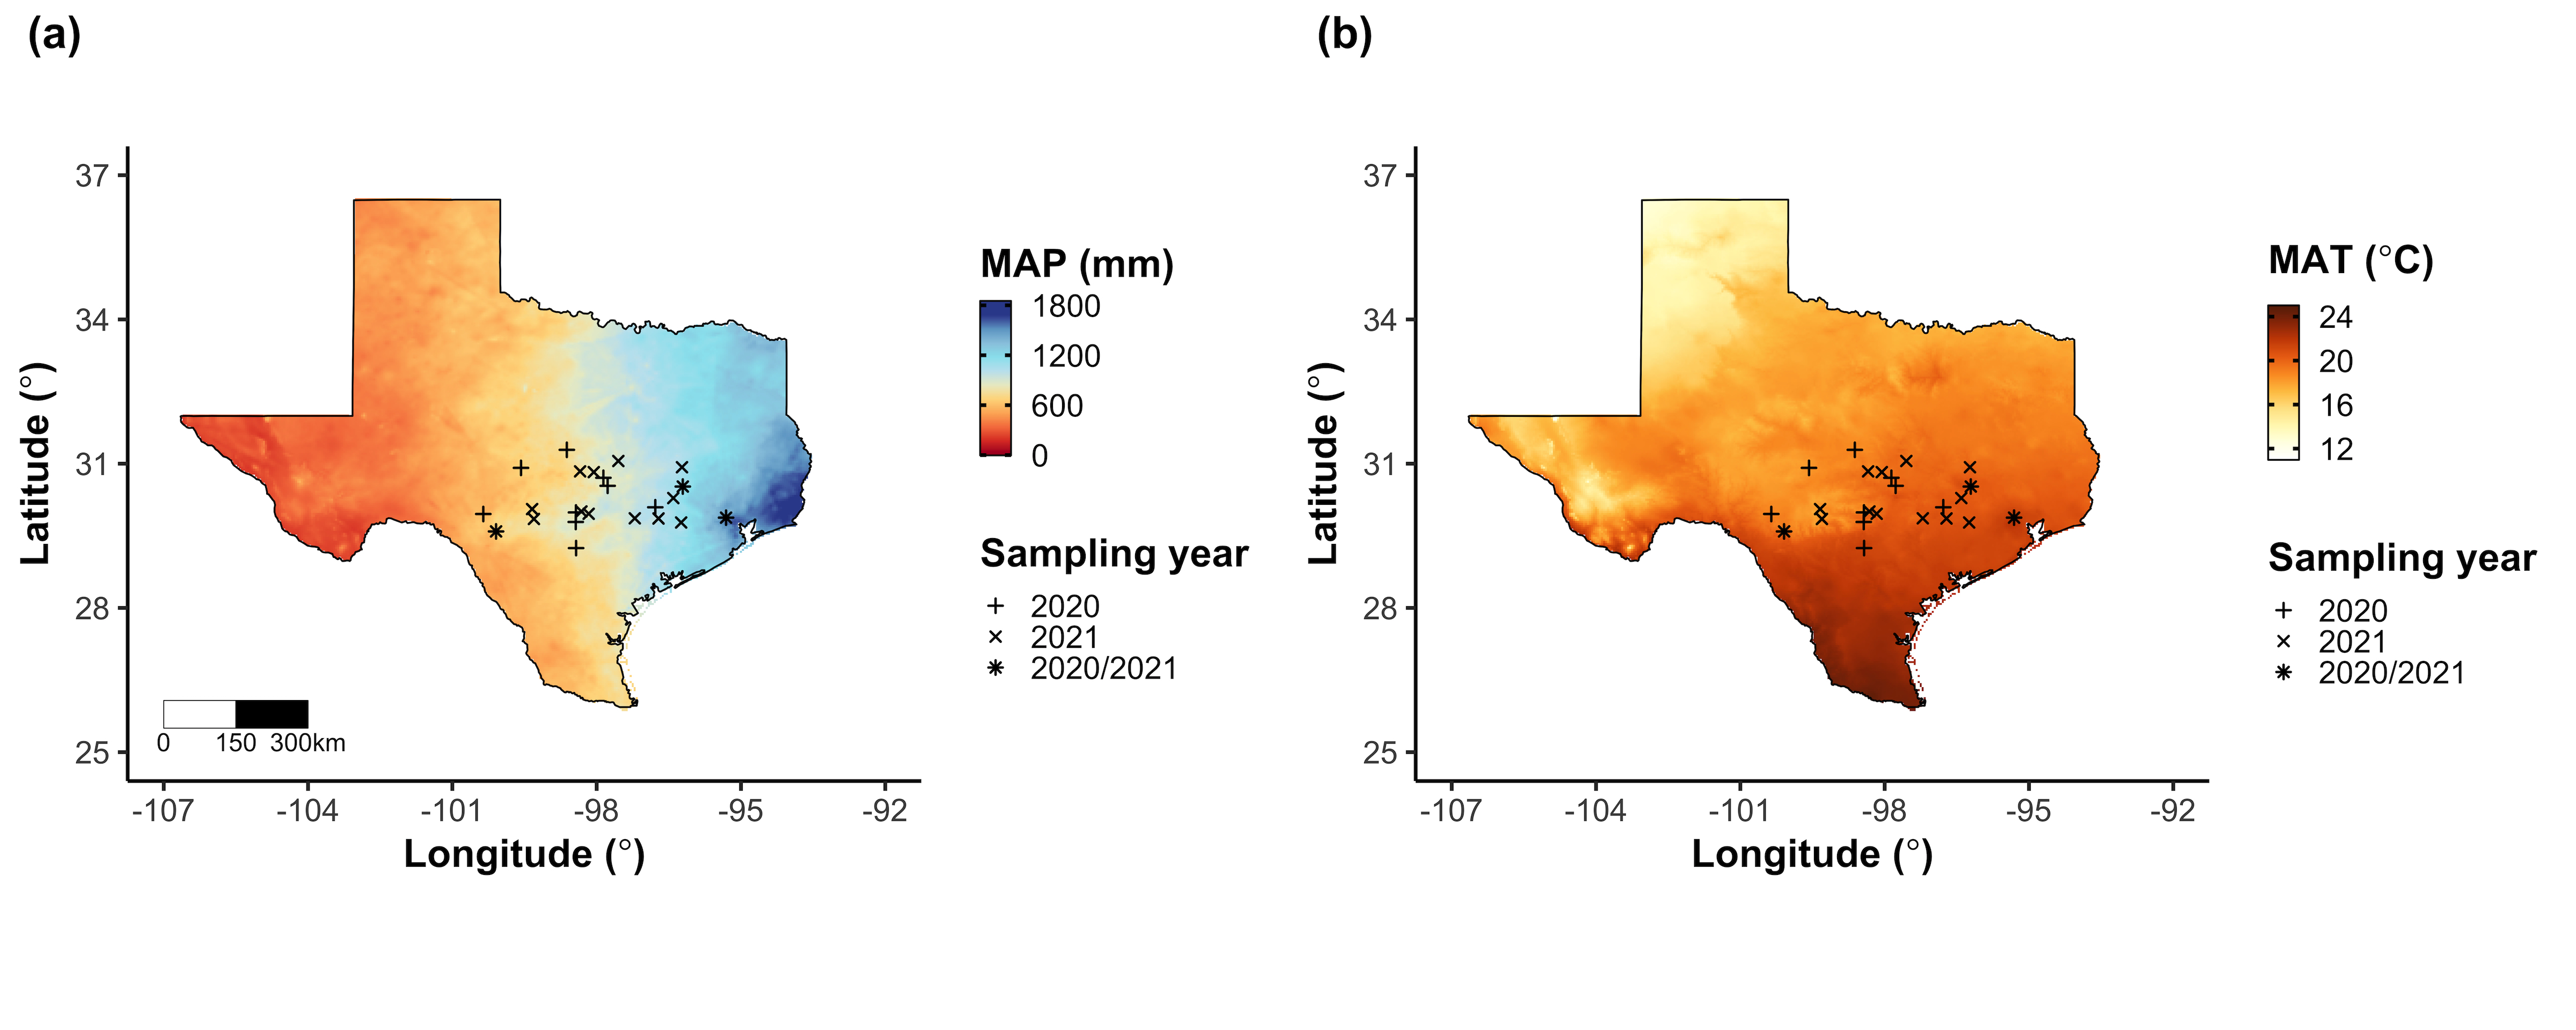
\includegraphics[width=\columnwidth]{ch4_TXeco/figs/TXeco_fig1_site_map.jpg}
        \caption[Site locations along 2006-2020 mean annual precipitation and mean annual temperature gradients in Texas, USA.]{Site locations along 2006-2020 mean annual precipitation (a) and mean annual temperature (b) gradients in Texas, USA. Precipitation and temperature data were plotted using PRISM data at a 4-km grid resolution and are masked to include only grid cells that occur within the Texas state boundary of the United States. In both panels, addition signs refer to sites visited in 2020, multiplication signs to sites visited in 2021, and asterisks to sites visited in 2020 and 2021. The scale bar in (a) also applies to (b).}
        \label{fig:figure4.1}
    \end{figure}
\end{landscape}
\clearpage

\subsection{\textit{Site climate data}}
\noindent I used the Parameter elevation Regressions on Independent Slopes Model (PRISM) \shortcite{Daly2008} climate product to access gridded daily temperature and precipitation data for the coterminous United States at a 4-km grid resolution between January 1, 2006 and July 31, 2021 (PRISM Climate Group, Oregon State University, \url{https://prism.oregonstate.edu}, data created 4 Feb 2014, accessed 24 Mar 2022). Mean daily air temperature, mean daily vapor pressure deficit, and total daily precipitation data were extracted from the grid cell that contained the latitude and longitude of each property using the `extract’ function in the `terra’ R package \shortcite{Hijmans2022}. PRISM data were used in lieu of local weather station data because several rural sites did not have a local weather station present within a 20-km radius of the site. Daily site climate data were used to estimate mean annual precipitation and mean annual temperature for each site between 2006 and 2020 (Table \ref{tab:table4.1}). I calculated total precipitation and mean daily vapor pressure deficit for the prior 1, 2, 3, 4, 5, 6, 7, 8, 9, 10, 15, 20, 25, 30, 60, and 90 days leading up to each site visit. Temperature was not included in any analysis due to the close range in mean annual temperature between sites (mean$\pm$SD: 19.8$\pm$0.9\textdegree{}C; Table \ref{tab:table4.1}).

\subsection{\textit{Site edaphic characteristics}}
\noindent Composited soil samples were sent to the Texas A\&M Soil, Water and Forage Laboratory to quantify soil nitrate concentration (NO$_3$-N; ppm). Soil NO$_3$-N was determined by extracting composite soil samples in 1 M KCl, measuring absorbance values of extracts at 520 nm using the end product of a NO$_3$-N to NO$_2$-N cadmium reduction reaction \shortcite{Kachurina2000,Keeney1983}. Soil texture data from 0-15 cm below the soil surface were accessed using the SoilGrids2.0 data product \shortcite{Poggio2021} through the `fetchSoilGrids’ function in the ‘soilDB’ R package \shortcite{Beaudette2022}. I used SoilGrids2.0 to access soil texture data in lieu of analyses using the composite soil sample due to a lack of soil material from some sites after sending samples for soil NO$_3$-N.

Soil moisture was estimated using the `Simple Process-Led Algorithms for Simulating Habitats’ model (SPLASH) \shortcite{Davis2017}. This model, derived from the STASH model \shortcite{Cramer1988}, initiates a bucket model using Priestley-Taylor equations \shortcite{Priestley1972} to calculate daily soil moisture ($W_\mathrm{n}$; mm) as a function of the previous day’s soil moisture ($W_\mathrm{n}{}_{-1}$; mm), daily precipitation ($P_\mathrm{n}$; mm), condensation ($C_\mathrm{n}$; mm), actual evapotranspiration ($E_{n}^a$; mm), and runoff (RO; mm):

\begin{equation}
    \label{eq_4.7}
    W_n = W_{n-1} + P_n + C_n - E_{n}^{a} - RO
\end{equation}

\noindent Models were initiated by equilibrating the previous day's soil moisture using successive model iterations with daily mean air temperature, daily precipitation total, the number of daily sunlight hours, and latitude as model inputs \shortcite{Davis2017}. Daily sunlight hours were estimated for each day at each site using the `getSunlightTimes’ function in the `suncalc’ R package, which estimated sunrise and sunset times of each property using date and site coordinates \shortcite{Thieurmel2019}. Water holding capacity (mm), or bucket size, was estimated as a function of soil texture using pedotransfer equations explained in \shortciteN{Saxton2006}, as done in \shortciteN{Stocker2020} and \shortciteN{Bloomfield2022}. A summary of these equations is included in \hyperref[appendix.c1]{Appendix C.1}.

Daily soil moisture outputs from the SPLASH model for each site were used to calculate mean daily soil moisture for the prior 1, 2, 3, 4, 5, 6, 7, 8, 9, 10, 15, 20, 25, 30, 60, and 90 days leading up to each site visit. Mean daily soil moisture values were then expressed as a fraction of water holding capacity to normalize across sites with different bucket depths, as done in \shortciteN{Stocker2018}. Site water holding capacity values are referenced in Table \ref{tab:table4.1}.

\subsection{\textit{Plant functional group assignments}}
\noindent Plant functional groups were assigned to each species and used as the primary descriptor of species identity. Specifically, plant functional groups were assigned based on photosynthetic pathway (C$_3$, C$_4$) and ability to form associations with symbiotic nitrogen-fixing bacteria (N-fixer, non-fixer). The ability to form associations with symbiotic nitrogen-fixing bacteria was assigned based on whether species were in the \textit{Fabaceae} family, and photosynthetic pathway of each species was determined from past literature and confirmed through leaf $\delta^{13}$C values. I chose these plant functional groups based on \textit{a priori} hypotheses regarding the functional role of nitrogen fixation and photosynthetic pathway on the sensitivity of plant nitrogen uptake and leaf nitrogen allocation to soil nitrogen availability and aboveground growing conditions. These plant functional group classifications resulted in three distinct plant functional groups within our dataset: C$_3$ N-fixers (n=53), C$_3$ non-fixers (n=334), and C$_4$ non-fixers (n=117).

\subsection{\textit{Data analysis}}
\noindent All analyses and plotting were conducted in R version 4.1.1 \shortcite{RCoreTeam2021}. I constructed a series of separate linear mixed-effects models to investigate environmental drivers of $\beta$, leaf $C_\mathrm{i}$:$C_\mathrm{a}$, $N_\mathrm{area}$, $N_\mathrm{mass}$, and $M_\mathrm{area}$, followed by a path analysis using a piecewise structural equation model to investigate direct and indirect effects of climate and soil resource availability on $N_\mathrm{area}$.

To explore environmental drivers of $\beta$, I built a linear mixed-effects model that included soil moisture, soil nitrogen availability, and plant functional group as fixed effect coefficients. Species were designated as a random intercept term. Interaction coefficients between all possible combinations of the three fixed effect coefficients were also included. $\beta$ was natural log transformed to linearize data. I used an information-theoretic model selection approach to determine whether 90-, 60-, 30-, 20-, 15-, 10-, 9-, 8-, 7-, 6-, 5-, 4-, 3-, 2-, or 1-day mean daily soil moisture conferred the best model fit for $\beta$. To do this, I constructed 16 separate linear mixed-effects models where log-transformed $\beta$ was included as the response variable and each soil moisture time step was separately included as a single continuous fixed effect. Species were included as a random intercept term for all models. I used corrected Akaike Information Criterion (AICc) to select the soil moisture timescale that conferred the best model fit, indicated by the model with the lowest AICc score (Table \ref{tab:tab.c4}; Fig. \ref{fig:figure.c1}).

To explore environmental drivers of leaf $C_\mathrm{i}$:$C_\mathrm{a}$, I constructed a second linear mixed effects model that included vapor pressure deficit, soil moisture, soil nitrogen availability, and plant functional group as fixed effect coefficients. Two-way interactions between plant functional group and vapor pressure deficit, soil nitrogen availability, or soil moisture were included as additional fixed effect coefficients, in addition to a three-way interaction between soil moisture, soil nitrogen availability, and plant functional group. Species were included as a random intercept term. I used an information-theoretic model selection approach to determine whether 90-, 60-, 30-, 20-, 15-, 10-, 9-, 8-, 7-, 6-, 5-, 4-, 3-, 2-, or 1-day mean daily vapor pressure deficit conferred the best model fit for leaf $C_\mathrm{i}$:$C_\mathrm{a}$ using the same approach explained above for the soil moisture effect on $\beta$. The soil moisture timescale was set to the same timescale that conferred the best fit for $\beta$.

To explore environmental drivers of $N_\mathrm{area}$, $N_\mathrm{mass}$, and $M_\mathrm{area}$, I constructed a linear mixed effects model for each trait, including leaf $C_\mathrm{i}$:$C_\mathrm{a}$, soil nitrogen availability, soil moisture, and plant functional group as fixed effect coefficients for each model. Two-way interactions between plant functional group and $\beta$, leaf $C_\mathrm{i}$:$C_\mathrm{a}$, soil nitrogen availability, or soil moisture were included as additional fixed effect coefficients, in addition to a three-way interaction between soil nitrogen availability, soil moisture, and plant functional group. Species were included as a random intercept term, with the soil moisture timescale set to the same timescale that conferred the best fit for $\beta$.

In all linear mixed-effects models explained above, including those to select relevant timescales, I used the `lmer' function in the `lme4' R package \shortcite{Bates2015} to fit each model and the `Anova' function in the `car' R package \shortcite{Fox2019} to calculate Type II Wald's $\chi^2$ and determine the significance level ($\alpha$=0.05) of each fixed effect coefficient. I used the `emmeans' R package \shortcite{Lenth2019} to conduct post-hoc comparisons using Tukey's tests, where degrees of freedom were approximated using the Kenward-Roger approach \shortcite{Kenward1997}. Trendlines and error ribbons for all plots were drawn using a series of `emmeans’ outputs across the range in plotted x-axis values.

Finally, I conducted a path analysis using a piecewise structural equation model to examine direct and indirect pathways that determined variance in $N_\mathrm{area}$. Six separate linear mixed effects models were loaded into the piecewise structural equation model. Models were constructed per \textit{a priori} hypotheses following patterns expected from photosynthetic least-cost theory. The first model regressed $N_\mathrm{area}$ against $N_\mathrm{mass}$ and $M_\mathrm{area}$. The second model regressed $M_\mathrm{area}$ against leaf $C_\mathrm{i}$:$C_\mathrm{a}$ and soil nitrogen availability. The third model regressed $N_\mathrm{mass}$ against leaf $C_\mathrm{i}$:$C_\mathrm{a}$ and $M_\mathrm{area}$ \shortcite{Dong2017,Dong2020}. The fourth model regressed leaf $C_\mathrm{i}$:$C_\mathrm{a}$ against $\beta$ and vapor pressure deficit. The fifth model regressed $\beta$ against soil nitrogen availability, soil moisture, ability to associate with symbiotic nitrogen-fixing bacteria, and photosynthetic pathway. The sixth model regressed soil nitrogen availability against soil moisture and percent clay to evaluate likely contributors of soil nitrogen availability. All models included the relevant timescale selected in the individual linear mixed effect models explained above. Models included species as a random intercept term, were built using the `lme’ function in the `nlme’ R package \shortcite{Pinheiro2022}, and subsequently loaded into the piecewise structural equation model using the `psem’ function in the `piecewiseSEM’ R package \shortcite{Lefcheck2016}.
\clearpage

\newpage
\section{Results}
\subsection{\textit{Cost to acquire nitrogen relative to water}}
\noindent Model selection indicated that 3-day mean soil moisture conferred the best model fit for $\beta$ (AICc=1870.10, RMSE=1.4135; Table \ref{tab:tab.c4}; Fig. \ref{fig:figure.c1}). An interaction between soil nitrogen availability and plant functional group (\textit{p}=0.005; Table \ref{tab:table4.2}) indicated that a negative effect of increasing soil nitrogen availability on $\beta$ was driven by a negative effect of increasing soil nitrogen on $\beta$ in C$_4$ non-fixers (Tukey: \textit{p}<0.001) and marginal negative effect in C$_3$ non-fixers (Tukey: \textit{p}=0.100), with no effect of soil nitrogen availability on $\beta$ in C$_3$ N-fixers (Tukey: \textit{p}=0.147; Table \ref{tab:table4.2}; Fig. \ref{fig:figure4.2}a). A second interaction between soil moisture and plant functional group (\textit{p}<0.001; Table \ref{tab:table4.2}) indicated that a negative effect of increasing soil moisture on $\beta$ (\textit{p}=0.002) was driven by C$_4$ non-fixers and null effects of soil moisture on $\beta$ in C$_3$ non-fixers (Tukey: \textit{p}=0.852) or C$_3$ N-fixers (Tukey: \textit{p}=0.650; Table \ref{tab:table4.2}; Fig. \ref{fig:figure4.2}b). A functional group effect (\textit{p}<0.001; Table \ref{tab:table4.2}) indicated that C$_4$ non-fixers had lower $\beta$ than both C$_3$ N-fixers and C$_3$ non-fixers (Tukey: \textit{p}<0.001 in both cases), while $\beta$ in C$_3$ N-fixers did not differ from C$_3$ non-fixers (Tukey: \textit{p}=0.628).

\newpage
\begin{table}
    \centering
    \caption[Effects of soil moisture, soil nitrogen availability, and plant functional group on $\beta$]{Effects of soil moisture, soil nitrogen availability, and plant functional group on $\beta$ (unitless)$^*$}
    %\resizebox{\columnwidth}{!}{
        \begin{tabular}{p{3.75cm}p{0.5cm}p{2cm}p{1.5cm}p{1.5cm}}
            \hline 
            & \multicolumn{1}{r}{df} 
            & \multicolumn{1}{r}{Coefficient} 
            & \multicolumn{1}{r}{$\chi^{2}$} 
            & \multicolumn{1}{r}{\textit{p}} 
            \\ 
            \hline
            
            Intercept
            & \multicolumn{1}{r}{-}
            & \multicolumn{1}{r}{$3.37*10^{0}$}
            & \multicolumn{1}{r}{-}
            & \multicolumn{1}{r}{-}
            \\

            Soil moisture (SM\textsubscript{3})
            & \multicolumn{1}{r}{1}
            & \multicolumn{1}{r}{$2.07*10^{-1}$}
            & \multicolumn{1}{r}{9.254}
            & \multicolumn{1}{r}{\textbf{0.002}}
            \\

            Soil N (N)
            & \multicolumn{1}{r}{1}
            & \multicolumn{1}{r}{$-1.67*10^{-2}$}
            & \multicolumn{1}{r}{14.547}
            & \multicolumn{1}{r}{\textbf{<0.001}}
            \\

            PFT
            & \multicolumn{1}{r}{2}
            & \multicolumn{1}{r}{-}
            & \multicolumn{1}{r}{408.426}
            & \multicolumn{1}{r}{\textbf{<0.001}}
            \\

            SM\textsubscript{3}*N
            & \multicolumn{1}{r}{1}
            & \multicolumn{1}{r}{$-4.03*10^{-3}$}
            & \multicolumn{1}{r}{0.134}
            & \multicolumn{1}{r}{0.714}
            \\

            SM\textsubscript{3}*PFT
            & \multicolumn{1}{r}{2}
            & \multicolumn{1}{r}{-}
            & \multicolumn{1}{r}{36.746}
            & \multicolumn{1}{r}{\textbf{<0.001}}
            \\

            N*PFT
            & \multicolumn{1}{r}{2}
            & \multicolumn{1}{r}{-}
            & \multicolumn{1}{r}{10.485}
            & \multicolumn{1}{r}{\textbf{0.005}}
            \\

            SM\textsubscript{3}*N*PFT
            & \multicolumn{1}{r}{2}
            & \multicolumn{1}{r}{-}
            & \multicolumn{1}{r}{1.324}
            & \multicolumn{1}{r}{0.516}
            \\
            \hline
        \end{tabular}%}
    \label{tab:table4.2}
\end{table}
\begin{singlespace}
    \noindent $^*$Significance determined using Type II Wald $\chi^{2}$ tests ($\alpha$=0.05). \textit{P}-values<0.05 are in bold. Model coefficients are expressed on the natural-log scale and are only included for continuous fixed effects. Key: df=degrees of freedom; $\chi^2$=Wald Type II chi-square test statistic
\end{singlespace}
\clearpage

\newpage
\begin{landscape}
    \begin{figure}
    \centering
    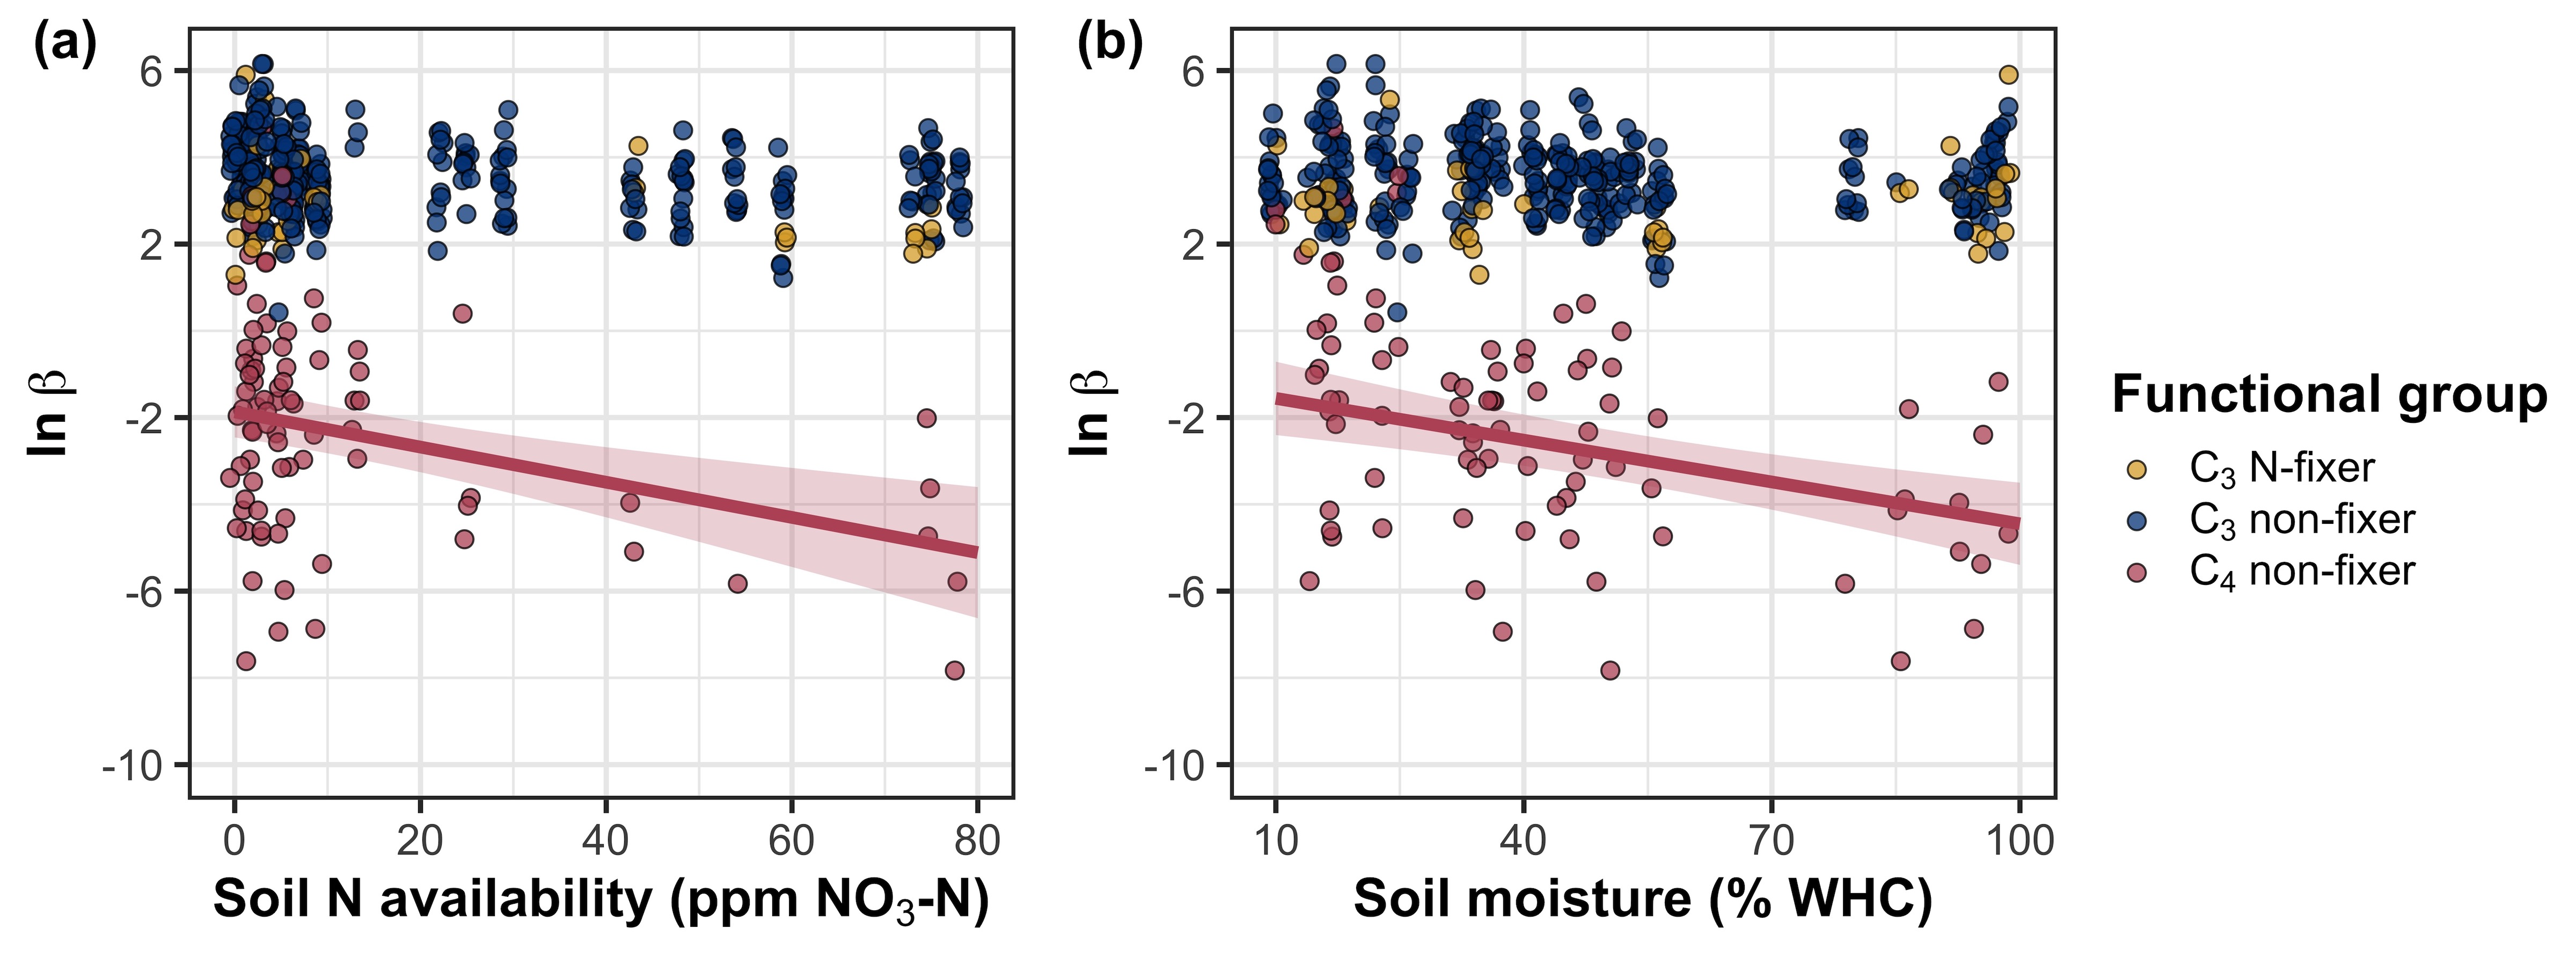
\includegraphics[width=\columnwidth]{ch4_TXeco/figs/TXeco_fig2_beta.jpg}
    \caption[Effects of soil nitrogen availability and soil moisture on the cost of acquiring and using nitrogen relative to water]{Effects of soil nitrogen availability (a) and soil moisture (b) on the cost of acquiring and using nitrogen relative to water ($\beta$; unitless). Soil nitrogen availability is represented on the x-axis in (a), soil moisture is represented on the x-axis in (b) as a percent of site water holding capacity, and natural-log transformed $\beta$ is represented on the y-axis for both panels. Yellow points represent C$_3$ N-fixers, blue points represent C$_3$ non-fixers, and red points represent C$_4$ non-fixers. Points are jittered along the x-axis for visibility. Colored trendlines note bivariate relationships within plant functional groups and are only included when the regression line slope is different from zero (\textit{p}<0.05). Error ribbons represent the upper and lower 95\% confidence interval range.}
    \label{fig:figure4.2}
\end{figure}
\end{landscape}
\clearpage

\subsection{\textit{Leaf $C_\mathrm{i}$:$C_\mathrm{a}$}}
\noindent 

Model selection indicated that 4-day mean vapor pressure deficit conferred the best model fit for leaf $C_\mathrm{i}$:$C_\mathrm{a}$ (AICc=-867.19; Table \ref{tab:tab.c4}; Fig. \ref{fig:figure.c1}). An interaction between vapor pressure deficit and plant functional group (\textit{p}=0.034; Table \ref{tab:table4.3}) revealed that the negative effect of increasing vapor pressure deficit on leaf $C_\mathrm{i}$:$C_\mathrm{a}$ (\textit{p}<0.001; Table \ref{tab:table4.3}) was driven by C$_3$ non-fixers (Tukey: \textit{p}<0.001) and C$_3$ N-fixers (Tukey: \textit{p}=0.040; Table \ref{tab:table4.3}; Fig. \ref{fig:figure4.3}a). An additional interaction between soil nitrogen availability and plant functional group (\textit{p}=0.005; Table \ref{tab:table4.3}) indicated a negative effect of increasing soil nitrogen availability on leaf $C_\mathrm{i}$:$C_\mathrm{a}$ in C$_4$ non-fixers (Tukey: \textit{p}=0.007), with no effect in C$_3$ non-fixers (Tukey: \textit{p}=0.660) or C$_3$ N-fixers (Tukey: \textit{p}=0.231; Fig. \ref{fig:figure4.3}c). There was no effect of soil moisture on leaf $C_\mathrm{i}$:$C_\mathrm{a}$ (Table \ref{tab:table4.3}; Fig. \ref{fig:figure4.3}b). A plant functional group effect (\textit{p}<0.001; Table \ref{tab:table4.3}) indicated that C$_4$ non-fixers had lower leaf $C_\mathrm{i}$:$C_\mathrm{a}$ than C$_3$ N-fixers and C$_3$ non-fixers (Tukey: \textit{p}<0.001 in both cases), with no difference between C$_3$ N-fixers and C$_3$ non-fixers (Tukey: \textit{p}=0.866).

\newpage
\begin{table}
    \centering
    \caption[Effects of soil moisture, soil nitrogen availability, and plant functional group on leaf $C_\mathrm{i}$:$C_\mathrm{a}$]{Effects of soil moisture, soil nitrogen availability, and plant functional group on leaf $C_\mathrm{i}$:$C_\mathrm{a}$ (unitless)$^*$}
    %\resizebox{\columnwidth}{!}{
        \begin{tabular}{p{6cm}p{0.5cm}p{2cm}p{1.5cm}p{1.5cm}}
            \hline 
            & \multicolumn{1}{r}{df} 
            & \multicolumn{1}{r}{Coefficient} 
            & \multicolumn{1}{r}{$\chi^{2}$} 
            & \multicolumn{1}{r}{\textit{p}} 
            \\ 
            \hline
            
            Intercept
            & \multicolumn{1}{r}{-}
            & \multicolumn{1}{r}{$1.08*10^{0}$}
            & \multicolumn{1}{r}{-}
            & \multicolumn{1}{r}{-}
            \\

            Vapor pressure deficit (VPD$_4$)
            & \multicolumn{1}{r}{1}
            & \multicolumn{1}{r}{$-2.59*10^{-1}$}
            & \multicolumn{1}{r}{14.042}
            & \multicolumn{1}{r}{\textbf{<0.001}}
            \\

            Soil moisture (SM$_{3}$)
            & \multicolumn{1}{r}{1}
            & \multicolumn{1}{r}{$-3.26*10^{-3}$}
            & \multicolumn{1}{r}{1.398}
            & \multicolumn{1}{r}{0.237}
            \\

            Soil N (N)
            & \multicolumn{1}{r}{1}
            & \multicolumn{1}{r}{$-1.40*10^{-3}$}
            & \multicolumn{1}{r}{0.708}
            & \multicolumn{1}{r}{0.400}
            \\

            PFT
            & \multicolumn{1}{r}{2}
            & \multicolumn{1}{r}{-}
            & \multicolumn{1}{r}{451.106}
            & \multicolumn{1}{r}{\textbf{<0.001}}
            \\

            SM$_{3}$*N
            & \multicolumn{1}{r}{1}
            & \multicolumn{1}{r}{$1.47*10^{-3}$}
            & \multicolumn{1}{r}{0.318}
            & \multicolumn{1}{r}{0.573}
            \\

            VPD$_{4}$*PFT
            & \multicolumn{1}{r}{2}
            & \multicolumn{1}{r}{-}
            & \multicolumn{1}{r}{6.737}
            & \multicolumn{1}{r}{\textbf{0.034}}
            \\

            SM$_{3}$*PFT
            & \multicolumn{1}{r}{2}
            & \multicolumn{1}{r}{-}
            & \multicolumn{1}{r}{3.890}
            & \multicolumn{1}{r}{0.143}
            \\

            N*PFT
            & \multicolumn{1}{r}{2}
            & \multicolumn{1}{r}{-}
            & \multicolumn{1}{r}{10.622}
            & \multicolumn{1}{r}{\textbf{0.005}}
            \\

            SM$_{90}$*N*PFT
            & \multicolumn{1}{r}{2}
            & \multicolumn{1}{r}{-}
            & \multicolumn{1}{r}{0.409}
            & \multicolumn{1}{r}{0.815}
            \\
            \hline
        \end{tabular}%}
    \label{tab:table4.3}
\end{table}
\begin{singlespace}
    \noindent $^*$Significance determined using Type II Wald $\chi^{2}$ tests ($\alpha$=0.05). \textit{P}-values less than 0.05 are in bold and \textit{p}-values where 0.05<\textit{p}<0.1 are italicized. Leaf $C_\mathrm{i}$:$C_\mathrm{a}$ was not transformed prior to model fitting, so model coefficients are reported on the response scale. Model coefficients are only included for continuous fixed effects. Key: df=degrees of freedom; $\chi^2$=Wald Type II chi-square test statistic
\end{singlespace}
\clearpage

\newpage
\begin{figure}
    \centering
    
\includegraphics[width=\textwidth]{ch4_TXeco/figs/TXeco_fig3_chi.jpg}
    \caption[Effects of 4-day mean vapor pressure deficit, 3-day soil moisture (per water holding capacity), and soil nitrogen availability on leaf $C_\mathrm{i}$:$C_\mathrm{a}$]{Effects of 4-day mean vapor pressure deficit (a), 3-day soil moisture (per water holding capacity; b), and soil nitrogen availability (c) on leaf $C_\mathrm{i}$:$C_\mathrm{a}$. Shading and trendlines are as explained in Figure \ref{fig:figure4.2}. Points are jittered for visibility. Variably colored trendlines are only included if there is an interaction between the x-axis and plant functional group, where solid trendlines indicate slopes that are different from zero (\textit{p}<0.05). Error ribbons represent the upper and lower 95\% confidence intervals of each fitted trendline.}
    \label{fig:figure4.3}
\end{figure}
\clearpage

\subsection{\textit{Leaf nitrogen content}}
\noindent An interaction between leaf $C_\mathrm{i}$:$C_\mathrm{a}$ and plant functional group (\textit{p}<0.001; Table \ref{tab:table4.4}) revealed that the negative effect of increasing leaf $C_\mathrm{i}$:$C_\mathrm{a}$ on $N_\mathrm{area}$ (\textit{p}=0.003; Table \ref{tab:table4.4}) was driven by negative effects of increasing leaf $C_\mathrm{i}$:$C_\mathrm{a}$ on $N_\mathrm{area}$ in C$_3$ non-fixers (Tukey: \textit{p}<0.001) and marginal negative effect in C$_3$ N-fixers (Tukey: \textit{p}=0.089; Fig. \ref{fig:figure4.4}a). An interaction between soil nitrogen availability and soil moisture (\textit{p}=0.019; Table \ref{tab:table4.4}) indicated that the positive effect of increasing soil nitrogen availability on $N_\mathrm{area}$ (\textit{p}=0.046; Table \ref{tab:table4.4}; Fig. \ref{fig:figure4.4}d) declined with increasing soil moisture despite no individual effect of soil moisture on $N_\mathrm{area}$ (\textit{p}=0.858; Table \ref{tab:table4.4}; Fig. \ref{fig:figure4.4}g). Specifically, there was at least a marginal positive effect of increasing soil nitrogen availability on $N_\mathrm{area}$ when soil moisture was between 10\% and 60\% of water holding capacity (Tukey: \textit{p}<0.1 in all cases), with no effect of soil nitrogen availability on $N_\mathrm{area}$ when soil moisture was greater than 65\% of water holding capacity (Tukey: \textit{p}>0.1 in all cases). Finally, a plant functional group effect (\textit{p}<0.001; Table \ref{tab:table4.4}) indicated that C$_4$ non-fixers had lower $N_\mathrm{area}$ compared to C$_3$ N-fixers (Tukey: \textit{p}<0.001) and C$_3$ non-fixers (Tukey: \textit{p}=0.011), while C$_3$ N-fixers had lower $N_\mathrm{area}$ compared to C$_3$ non-fixers (Tukey: \textit{p}=0.020).

Leaf $C_\mathrm{i}$:$C_\mathrm{a}$ had no effect on $N_\mathrm{mass}$ (\textit{p}=0.943; Table \ref{tab:table4.4}; Fig. \ref{fig:figure4.4}b), though a marginal interaction between leaf $C_\mathrm{i}$:$C_\mathrm{a}$ and plant functional group (\textit{p}=0.065; Table \ref{tab:table4.4}) indicated a marginal negative effect of increasing leaf $C_\mathrm{i}$:$C_\mathrm{a}$ in C$_3$ non-fixers (Tukey: \textit{p}=0.094). An interaction between soil nitrogen availability and soil moisture (\textit{p}<0.001; Table \ref{tab:table4.4}) revealed that the positive effect of increasing soil nitrogen availability (\textit{p}<0.001; Table \ref{tab:table4.4}; Fig. \ref{fig:figure4.4}e) declined with increasing soil moisture. Specifically, this interaction indicated that the positive effect of increasing soil nitrogen availability on $N_\mathrm{mass}$ was only apparent when soil moisture was equal to or less than 70\% of water holding capacity (Tukey: \textit{p}<0.05 in all cases). Increasing soil moisture also generally increased $N_\mathrm{mass}$ (\textit{p}<0.001; Table \ref{tab:table4.4}; Fig. \ref{fig:figure4.4}h). A plant functional group effect (\textit{p}<0.001; Table \ref{tab:table4.4}) indicated that C$_4$ non-fixers had lower $N_\mathrm{mass}$ compared to C$_3$ N-fixers (Tukey: \textit{p}=0.006) and C$_3$ non-fixers (Tukey: \textit{p}=0.026 in both cases), while $N_\mathrm{mass}$ did not differ between C$_3$ N-fixers and C$_3$ non-fixers (Tukey: \textit{p}=0.293).

An interaction between leaf $C_\mathrm{i}$:$C_\mathrm{a}$ and plant functional group (\textit{p}<0.001; Table \ref{tab:table4.4}) revealed that the negative effect of increasing leaf $C_\mathrm{i}$:$C_\mathrm{a}$ on $M_\mathrm{area}$ (\textit{p}=0.002; Table \ref{tab:table4.4}) was driven by negative effects of increasing leaf $C_\mathrm{i}$:$C_\mathrm{a}$ on $M_\mathrm{area}$ in C$_3$ N-fixers (Tukey: \textit{p}<0.001) and C$_3$ non-fixers (Tukey: \textit{p}=0.004; Fig. \ref{fig:figure4.4}c). An interaction between soil nitrogen availability and plant functional group (\textit{p}=0.028; Table \ref{tab:table4.4}) indicated that the negative effect of increasing soil nitrogen availability on $M_\mathrm{area}$ (\textit{p}<0.001; Table \ref{tab:table4.4}) was driven by negative effects of increasing soil nitrogen availability on $M_\mathrm{area}$ in C$_4$ non-fixers (Tukey: \textit{p}=0.009) and C$_3$ non-fixers (Tukey: \textit{p}<0.001; Fig. \ref{fig:figure4.4}f). A third interaction between soil nitrogen availability and soil moisture (\textit{p}<0.001; Table \ref{tab:table4.4}) indicated that the negative effect of increasing soil nitrogen availability on $M_\mathrm{area}$ (\textit{p}<0.001; Table \ref{tab:table4.4}) diminished with increasing soil moisture due to a negative individual effect of increasing soil moisture on $M_\mathrm{area}$ (\textit{p}=0.006; Table \ref{tab:table4.4}; Fig. \ref{fig:figure4.4}i). This interaction indicated that the negative effect of increasing soil nitrogen availability on $M_\mathrm{area}$ was only apparent when soil moisture was equal to or less than 65\% of water holding capacity (Tukey: \textit{p}<0.05 in all cases). Increasing soil moisture generally 

\newpage
\begin{landscape}
    \begin{table}
    \centering
    \caption[Effects of soil moisture, soil nitrogen availability, plant functional group, and leaf $C_\mathrm{i}$:$C_\mathrm{a}$ on leaf nitrogen content per unit leaf area, leaf nitrogen content per unit leaf biomass, and leaf biomass per unit leaf area]{Effects of soil moisture, soil nitrogen availability, plant functional group, and leaf $C_\mathrm{i}$:$C_\mathrm{a}$ on leaf nitrogen content per unit leaf area ($N_\mathrm{area}$; gN m$^{-2}$), leaf nitrogen content per unit leaf biomass ($N_\mathrm{mass}$; gN g$^{-1}$), and leaf biomass per unit leaf area ($M_\mathrm{area}$; g m$^{-2}$)}
    \resizebox{\columnwidth}{!}{
        \begin{tabular}{p{3.75cm}p{0.5cm}p{1.75cm}p{1.5cm}p{1.5cm}p{1.75cm}p{1.5cm}p{1.5cm}p{1.75cm}p{1.5cm}p{1.5cm}}
            && 
            \multicolumn{3}{l}{$N_\mathrm{area}$} 
            & \multicolumn{3}{l}{$N_\mathrm{mass}$} 
            & \multicolumn{3}{l}{$M_\mathrm{area}$} 
            \\
            \hline 
            & 
            \multicolumn{1}{r}{df} 
            & \multicolumn{1}{r}{Coefficient}   & \multicolumn{1}{r}{$\chi^2$}    & \multicolumn{1}{r}{\textit{p}} 
            & \multicolumn{1}{r}{Coefficient}   & \multicolumn{1}{r}{$\chi^2$}    & \multicolumn{1}{r}{\textit{p}} 
            & \multicolumn{1}{r}{Coefficient}   & \multicolumn{1}{r}{$\chi^2$}    & \multicolumn{1}{r}{\textit{p}} 
            \\ 
            \hline

            (Intercept) & \multicolumn{1}{r}{-} 
            &  \multicolumn{1}{r}{$1.96*10^{0}$}     & \multicolumn{1}{r}{-}             & \multicolumn{1}{r}{-}
            &  \multicolumn{1}{r}{$1.772*10^{-1}$}   & \multicolumn{1}{r}{-}             & \multicolumn{1}{r}{-}
            &  \multicolumn{1}{r}{$6.42*10^{0}$}     & \multicolumn{1}{r}{-}             & \multicolumn{1}{r}{-} 
            \\

            $C_\mathrm{i}$:$C_\mathrm{a}$ & \multicolumn{1}{r}{1}
            & \multicolumn{1}{r}{$-1.31*10^{0}$}     & \multicolumn{1}{r}{4.387}         & \multicolumn{1}{r}{\textbf{0.036}}
            & \multicolumn{1}{r}{$8.05*10^{-1}$}    & \multicolumn{1}{r}{0.005}         & \multicolumn{1}{r}{0.943}
            & \multicolumn{1}{r}{$-2.21*10^{0}$}     & \multicolumn{1}{r}{9.673}        & \multicolumn{1}{r}{\textbf{0.002}} 
            \\ % updated


            Soil N (N) & \multicolumn{1}{r}{1}
            & \multicolumn{1}{r}{$1.18*10^{-2}$}    & \multicolumn{1}{r}{3.972}         & \multicolumn{1}{r}{\textbf{0.046}}
            & \multicolumn{1}{r}{$1.35*10^{-2}$}    & \multicolumn{1}{r}{49.093}        & \multicolumn{1}{r}{\textbf{<0.001}}
            & \multicolumn{1}{r}{$-1.59*10^{-3}$}   & \multicolumn{1}{r}{24.314}        & \multicolumn{1}{r}{\textbf{<0.001}} 
            \\ % updated

            Soil moisture (SM$_{3}$) & \multicolumn{1}{r}{1}
            & \multicolumn{1}{r}{$3.79*10^{-1}$}      & \multicolumn{1}{r}{0.032}         & \multicolumn{1}{r}{0.858}
            & \multicolumn{1}{r}{$5.07*10^{-1}$}      & \multicolumn{1}{r}{11.443}        & \multicolumn{1}{r}{\textbf{<0.001}}
            & \multicolumn{1}{r}{$-9.92*10^{-2}$}     & \multicolumn{1}{r}{7.649}         & \multicolumn{1}{r}{\textbf{0.006}} 
            \\ % updated

            PFT & \multicolumn{1}{r}{1}
            & \multicolumn{1}{r}{-}             & \multicolumn{1}{r}{43.761}        & \multicolumn{1}{r}{\textbf{<0.001}}
            & \multicolumn{1}{r}{-}             & \multicolumn{1}{r}{19.758}        & \multicolumn{1}{r}{\textbf{<0.001}}
            & \multicolumn{1}{r}{-}             & \multicolumn{1}{r}{10.168}         & \multicolumn{1}{r}{\textbf{0.006}} 
            \\ % updated

            SM$_{3}$*N & \multicolumn{1}{r}{1}
            & \multicolumn{1}{r}{$-1.27*10^{-2}$}     & \multicolumn{1}{r}{5.521}         & \multicolumn{1}{r}{\textbf{0.019}}
            & \multicolumn{1}{r}{$-1.80*10^{-2}$}     & \multicolumn{1}{r}{44.013}        & \multicolumn{1}{r}{\textbf{<0.001}}
            & \multicolumn{1}{r}{$4.79*10^{-3}$}      & \multicolumn{1}{r}{14.195}        & \multicolumn{1}{r}{\textbf{<0.001}} 
            \\ % updated

            $C_\mathrm{i}$:$C_\mathrm{a}$*PFT & \multicolumn{1}{r}{1}
            & \multicolumn{1}{r}{-}             & \multicolumn{1}{r}{17.302}        & \multicolumn{1}{r}{\textbf{<0.001}}
            & \multicolumn{1}{r}{-}             & \multicolumn{1}{r}{5.471}         & \multicolumn{1}{r}{\textit{ 0.065}}
            & \multicolumn{1}{r}{-}             & \multicolumn{1}{r}{13.974}        & \multicolumn{1}{r}{\textbf{<0.001}} 
            \\ % updated

            N*PFT & \multicolumn{1}{r}{1}
            & \multicolumn{1}{r}{-}             & \multicolumn{1}{r}{1.540}         & \multicolumn{1}{r}{0.463}
            & \multicolumn{1}{r}{-}             & \multicolumn{1}{r}{1.047}         & \multicolumn{1}{r}{0.592}
            & \multicolumn{1}{r}{-}             & \multicolumn{1}{r}{7.182}         & \multicolumn{1}{r}{\textbf{0.028}}
            \\ % updated

            SM\textsubscript{3}*PFT & \multicolumn{1}{r}{1}
            & \multicolumn{1}{r}{-}             & \multicolumn{1}{r}{1.113}         & \multicolumn{1}{r}{0.573}
            & \multicolumn{1}{r}{-}             & \multicolumn{1}{r}{2.004}         & \multicolumn{1}{r}{0.367}
            & \multicolumn{1}{r}{-}             & \multicolumn{1}{r}{3.785}         & \multicolumn{1}{r}{0.151} 
            \\

            SM$_{3}$*N*PFT & \multicolumn{1}{r}{1}
            & \multicolumn{1}{r}{-}             & \multicolumn{1}{r}{0.632}         & \multicolumn{1}{r}{0.729}
            & \multicolumn{1}{r}{-}             & \multicolumn{1}{r}{0.895}         & \multicolumn{1}{r}{0.639}
            & \multicolumn{1}{r}{-}             & \multicolumn{1}{r}{0.913}         & \multicolumn{1}{r}{0.634}
            \\
            \hline

    \end{tabular}}
    \label{tab:table4.4}
\end{table}
\begin{singlespace}
    \noindent \textsuperscript{$*$}Significance determined using Type II Wald $\chi^{2}$ tests ($\alpha$=0.05). \textit{P}-values less than 0.05 are in bold and \textit{p}-values where 0.05<\textit{p}<0.1 are italicized. Coefficients are reported on the natural-log scale for all traits and are only included for continuous fixed effects. Key: df=degrees of freedom; $\chi^2$=Wald Type II chi-square test statistic
\end{singlespace}
\end{landscape}
\clearpage

\newpage
    \begin{figure}
        \centering
        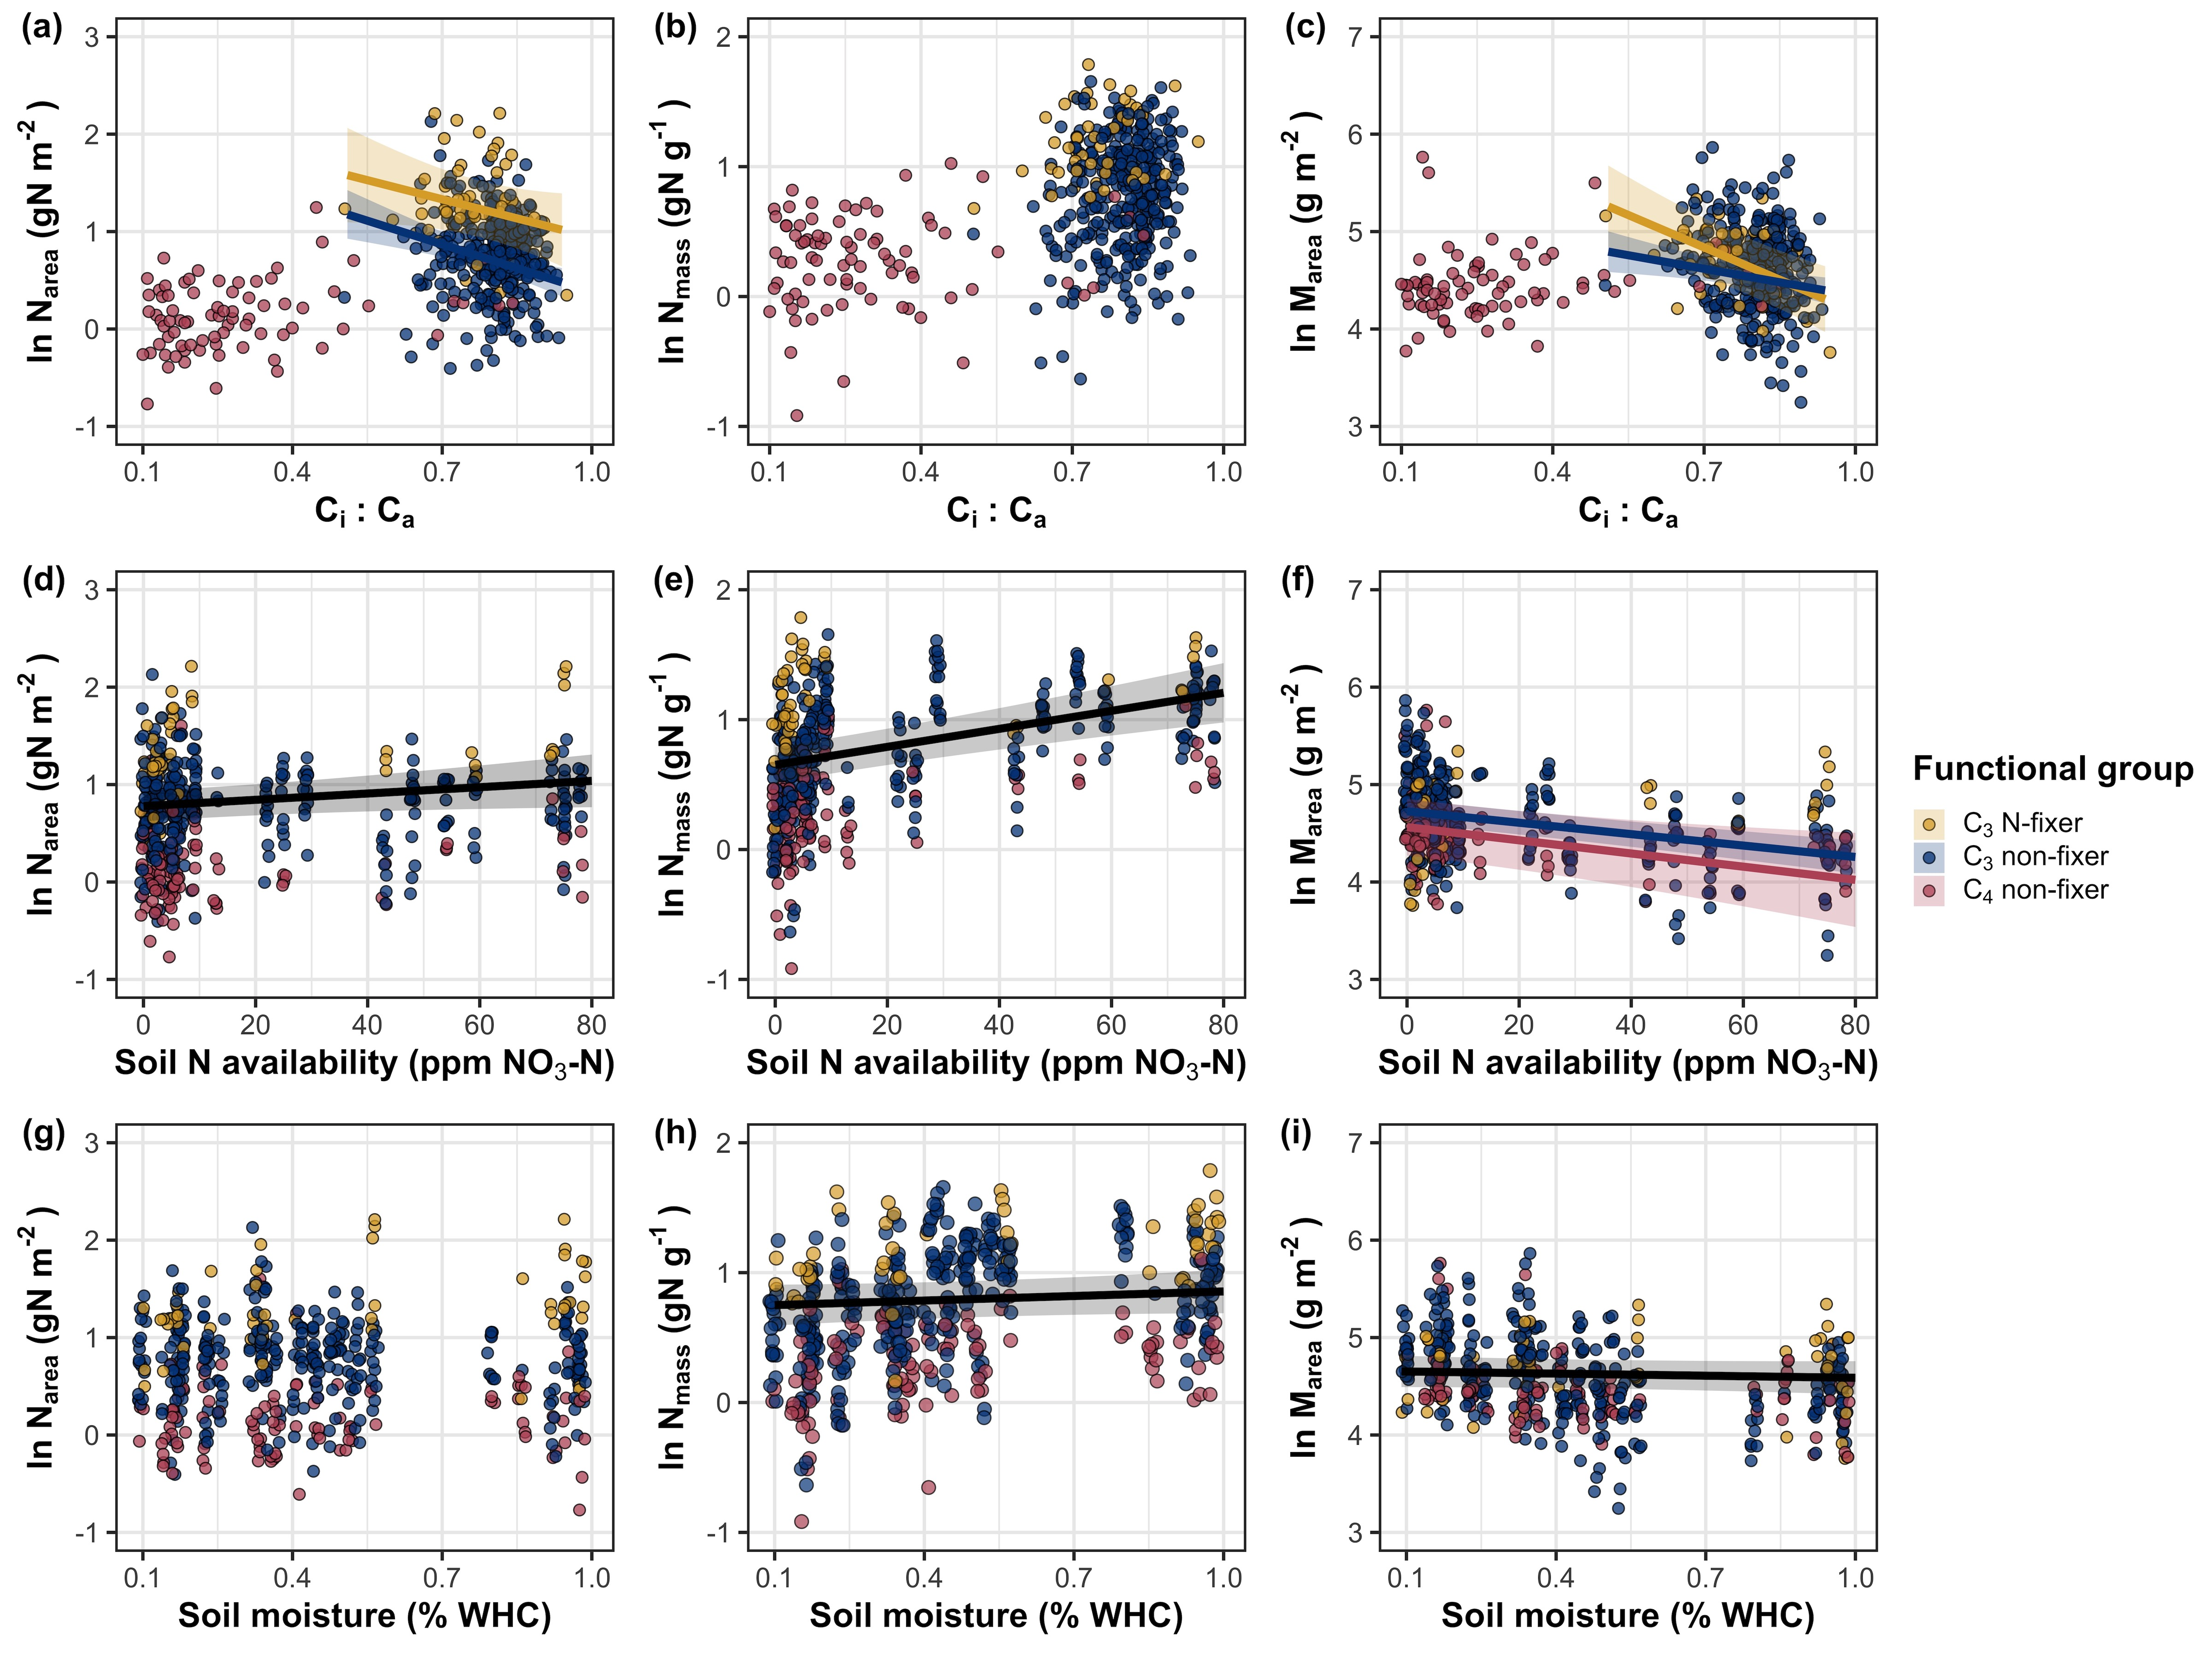
\includegraphics[width=\textwidth]{ch4_TXeco/figs/TXeco_fig4_narea.jpg}
        \caption[Effects of leaf $C_\mathrm{i}$:$C_\mathrm{a}$, soil nitrogen availability, and soil moisture on leaf nitrogen content per unit leaf area, leaf nitrogen content per unit leaf biomass, and leaf mass per area.]{Effects of leaf $C_\mathrm{i}$:$C_\mathrm{a}$ (a-c), soil nitrogen availability (d-f), and soil moisture (g-i) on leaf nitrogen content per unit leaf area (a, d, g), leaf nitrogen content per unit leaf biomass (b, e, h), and leaf mass per area (c, f, i). Yellow points and trendlines indicate C$_3$ N-fixers, blue points and trendlines indicate C$_3$ non-fixers, and red points and trendlines indicate C$_4$ non-fixers. Points are jittered for visibility. Variably colored trendlines are only included if there is an interaction between plant functional group and the x-axis. Black solid trendlines denote bivariate slopes that are different from zero (\textit{p}<0.05) where there is no apparent interaction between plant functional group and the x-axis.}
        \label{fig:figure4.4}
    \end{figure}
\clearpage

\subsection{\textit{Structural equation model}}
\noindent The piecewise structural equation model explained 89\%, 56\%, 58\%, 93\%, and 28\% of variance in $N_\mathrm{area}$, $N_\mathrm{mass}$, $M_\mathrm{area}$, leaf $C_\mathrm{i}$:$C_\mathrm{a}$, and $\beta$, respectively (Table \ref{tab:table4.5}; Fig. \ref{fig:figure4.5}). Increasing $N_\mathrm{mass}$ and $M_\mathrm{area}$ were each positively related to $N_\mathrm{area}$ (\textit{p}<0.001 in both cases; Table \ref{tab:table4.5}; Fig. \ref{fig:figure4.5}). $N_\mathrm{mass}$ increased with increasing soil nitrogen availability (\textit{p}<0.001; Table \ref{tab:table4.5}) and leaf $C_\mathrm{i}$:$C_\mathrm{a}$ (\textit{p}=0.001; Table \ref{tab:table4.5}), and was generally larger in N-fixing species (\textit{p}<0.001; Table \ref{tab:table4.5}), but was negatively related to increasing $M_\mathrm{area}$ (\textit{p}<0.001; Table \ref{tab:table4.5}). $M_\mathrm{area}$ decreased with increasing leaf $C_\mathrm{i}$:$C_\mathrm{a}$ (\textit{p}=0.019 in both cases; Table \ref{tab:table4.5}) and soil nitrogen availability (\textit{p}<0.001; Table \ref{tab:table4.5}). Leaf $C_\mathrm{i}$:$C_\mathrm{a}$ declined with increasing vapor pressure deficit, but was positively related to $\beta$ (\textit{p}<0.001 in both cases; Table \ref{tab:table4.5}). $\beta$ decreased with increasing soil nitrogen availability (\textit{p}=0.001; Table \ref{tab:table4.5}) and was greater in C$_3$ species (\textit{p}<0.001; Table \ref{tab:table4.5}), but did not change with soil moisture (\textit{p}=0.915; Table \ref{tab:table4.5}) or with ability to acquire nitrogen via symbiotic nitrogen fixation (\textit{p}=0.306; Table \ref{tab:table4.5}). Finally, soil nitrogen availability was positively associated with increasing soil moisture (\textit{p}<0.001; Table \ref{tab:table4.5}; Fig. \ref{fig:figure4.5}), while soil moisture was negatively related to percent clay (\textit{p}<0.001; Table \ref{tab:table4.5}; Fig. \ref{fig:figure4.5}).

\newpage
\begin{table}
    \centering
    \caption[Structural equation model results investigating direct effects of climatic and soil resource availability on leaf nitrogen content]{Structural equation model results investigating direct effects of climatic and soil resource availability on leaf nitrogen content ($N_\mathrm{area}$; g m$^{-2}$)$^*$}
    %\resizebox{\columnwidth}{!}{
        \begin{tabular}{p{0.5cm}p{3cm}p{1.5cm}p{1.5cm}}
            \hline
            & Predictor & \multicolumn{1}{r}{Coefficient} & \multicolumn{1}{r}{\textit{p}} \\
            \hline

            \multicolumn{2}{l}{$N_\mathrm{area}$ ($R^2{}_\mathrm{c}$=0.89)} && \\
            & \multicolumn{1}{l}{$M_\mathrm{area}$} & \multicolumn{1}{r}{0.713}     & \multicolumn{1}{r}{\textbf{<0.001}} \\
            & \multicolumn{1}{l}{$N_\mathrm{mass}$} & \multicolumn{1}{r}{0.787}     & \multicolumn{1}{r}{\textbf{<0.001}} \\
            \hline

            \multicolumn{2}{l}{$N_\mathrm{mass}$ ($R^2{}_\mathrm{c}$=0.56)} && \\
            & \multicolumn{1}{l}{Leaf $C_\mathrm{i}$:$C_\mathrm{a}$}    & \multicolumn{1}{r}{0.207}     & \multicolumn{1}{r}{\textbf{0.001}} \\
            & \multicolumn{1}{l}{$M_\mathrm{area}$}                     & \multicolumn{1}{r}{-0.240}    & \multicolumn{1}{r}{\textbf{<0.001}} \\
            & \multicolumn{1}{l}{Soil N}                                & \multicolumn{1}{r}{0.242}     & \multicolumn{1}{r}{\textbf{<0.001}} \\
            & \multicolumn{1}{l}{N-fixing ability}                      & \multicolumn{1}{r}{0.335}     & \multicolumn{1}{r}{\textbf{<0.001}} \\
            \hline

            \multicolumn{2}{l}{$M_\mathrm{area}$ ($R^2{}_\mathrm{c}$=0.58)} && \\
            & \multicolumn{1}{l}{Leaf $C_\mathrm{i}$:$C_\mathrm{a}$}    & \multicolumn{1}{r}{-0.187}    & \multicolumn{1}{r}{\textbf{0.019}} \\
            & \multicolumn{1}{l}{Soil N}                                & \multicolumn{1}{r}{-0.209}    & \multicolumn{1}{r}{\textbf{<0.001}} \\
            \hline

            \multicolumn{2}{l}{Leaf $C_\mathrm{i}$:$C_\mathrm{a}$ ($R^2{}_\mathrm{c}$=0.93)} && \\
            & \multicolumn{1}{l}{$\beta$}                               & \multicolumn{1}{r}{0.154}     & \multicolumn{1}{r}{\textbf{<0.001}} \\
            & \multicolumn{1}{l}{VPD$_4$}                               & \multicolumn{1}{r}{-0.082}    & \multicolumn{1}{r}{\textbf{<0.001}} \\
            \hline

            \multicolumn{2}{l}{$\beta$ ($R^2{}_\mathrm{c}$=0.28)} && \\
            & \multicolumn{1}{l}{Soil N}                                & \multicolumn{1}{r}{-0.161}    & \multicolumn{1}{r}{\textbf{0.001}} \\
            & \multicolumn{1}{l}{SM$_{3}$}                             & \multicolumn{1}{r}{-0.006}    & \multicolumn{1}{r}{0.915} \\
            & \multicolumn{1}{l}{Photo. pathway}                        & \multicolumn{1}{r}{0.417}     & \multicolumn{1}{r}{\textbf{<0.001}} \\
            & \multicolumn{1}{l}{N-fixing ability}                      & \multicolumn{1}{r}{-0.082}    & \multicolumn{1}{r}{0.306} \\
            \hline

            \multicolumn{2}{l}{Soil N ($R^2{}_\mathrm{c}$=0.41)} && \\
            & \multicolumn{1}{l}{SM$_{3}$} & \multicolumn{1}{r}{-0.409} & \multicolumn{1}{r}{\textbf{<0.001}} \\
            \hline

            \multicolumn{2}{l}{Soil moisture ($R^2{}_\mathrm{c}$=0.51)} && \\
            & \multicolumn{1}{l}{\% clay} & \multicolumn{1}{r}{-0.433} & \multicolumn{1}{r}{\textbf{<0.001}} \\
            \hline

        \end{tabular}%}
        \label{tab:table4.5}
    \end{table}
\begin{singlespace}
    \noindent $^*$Coefficients are standardized across the structural equation model. \textit{P}-values less than 0.05 are noted in bold. Positive coefficients for photosynthetic pathway indicate generally larger values in C$_3$ species, while positive coefficients for N-fixing ability indicate generally larger values in N-fixing species. Key: df=degrees of freedom; $\chi^2$=Wald Type II chi-square test statistic; $R^2{}_\mathrm{c}$=conditional R$^2$ value; $N_\mathrm{mass}$=leaf nitrogen content per unit leaf biomass (gN g$^{-1}$); $M_\mathrm{area}$=leaf mass per unit leaf biomass (g m$^{-2}$); $\beta$=cost of acquiring nitrogen relative to water (unitless); VPD$_4$=4-day mean vapor pressure deficit (kPa); SM$_{90}$=90-day mean soil moisture (mm)
\end{singlespace}
\clearpage

\newpage
    \begin{figure}
        \centering
        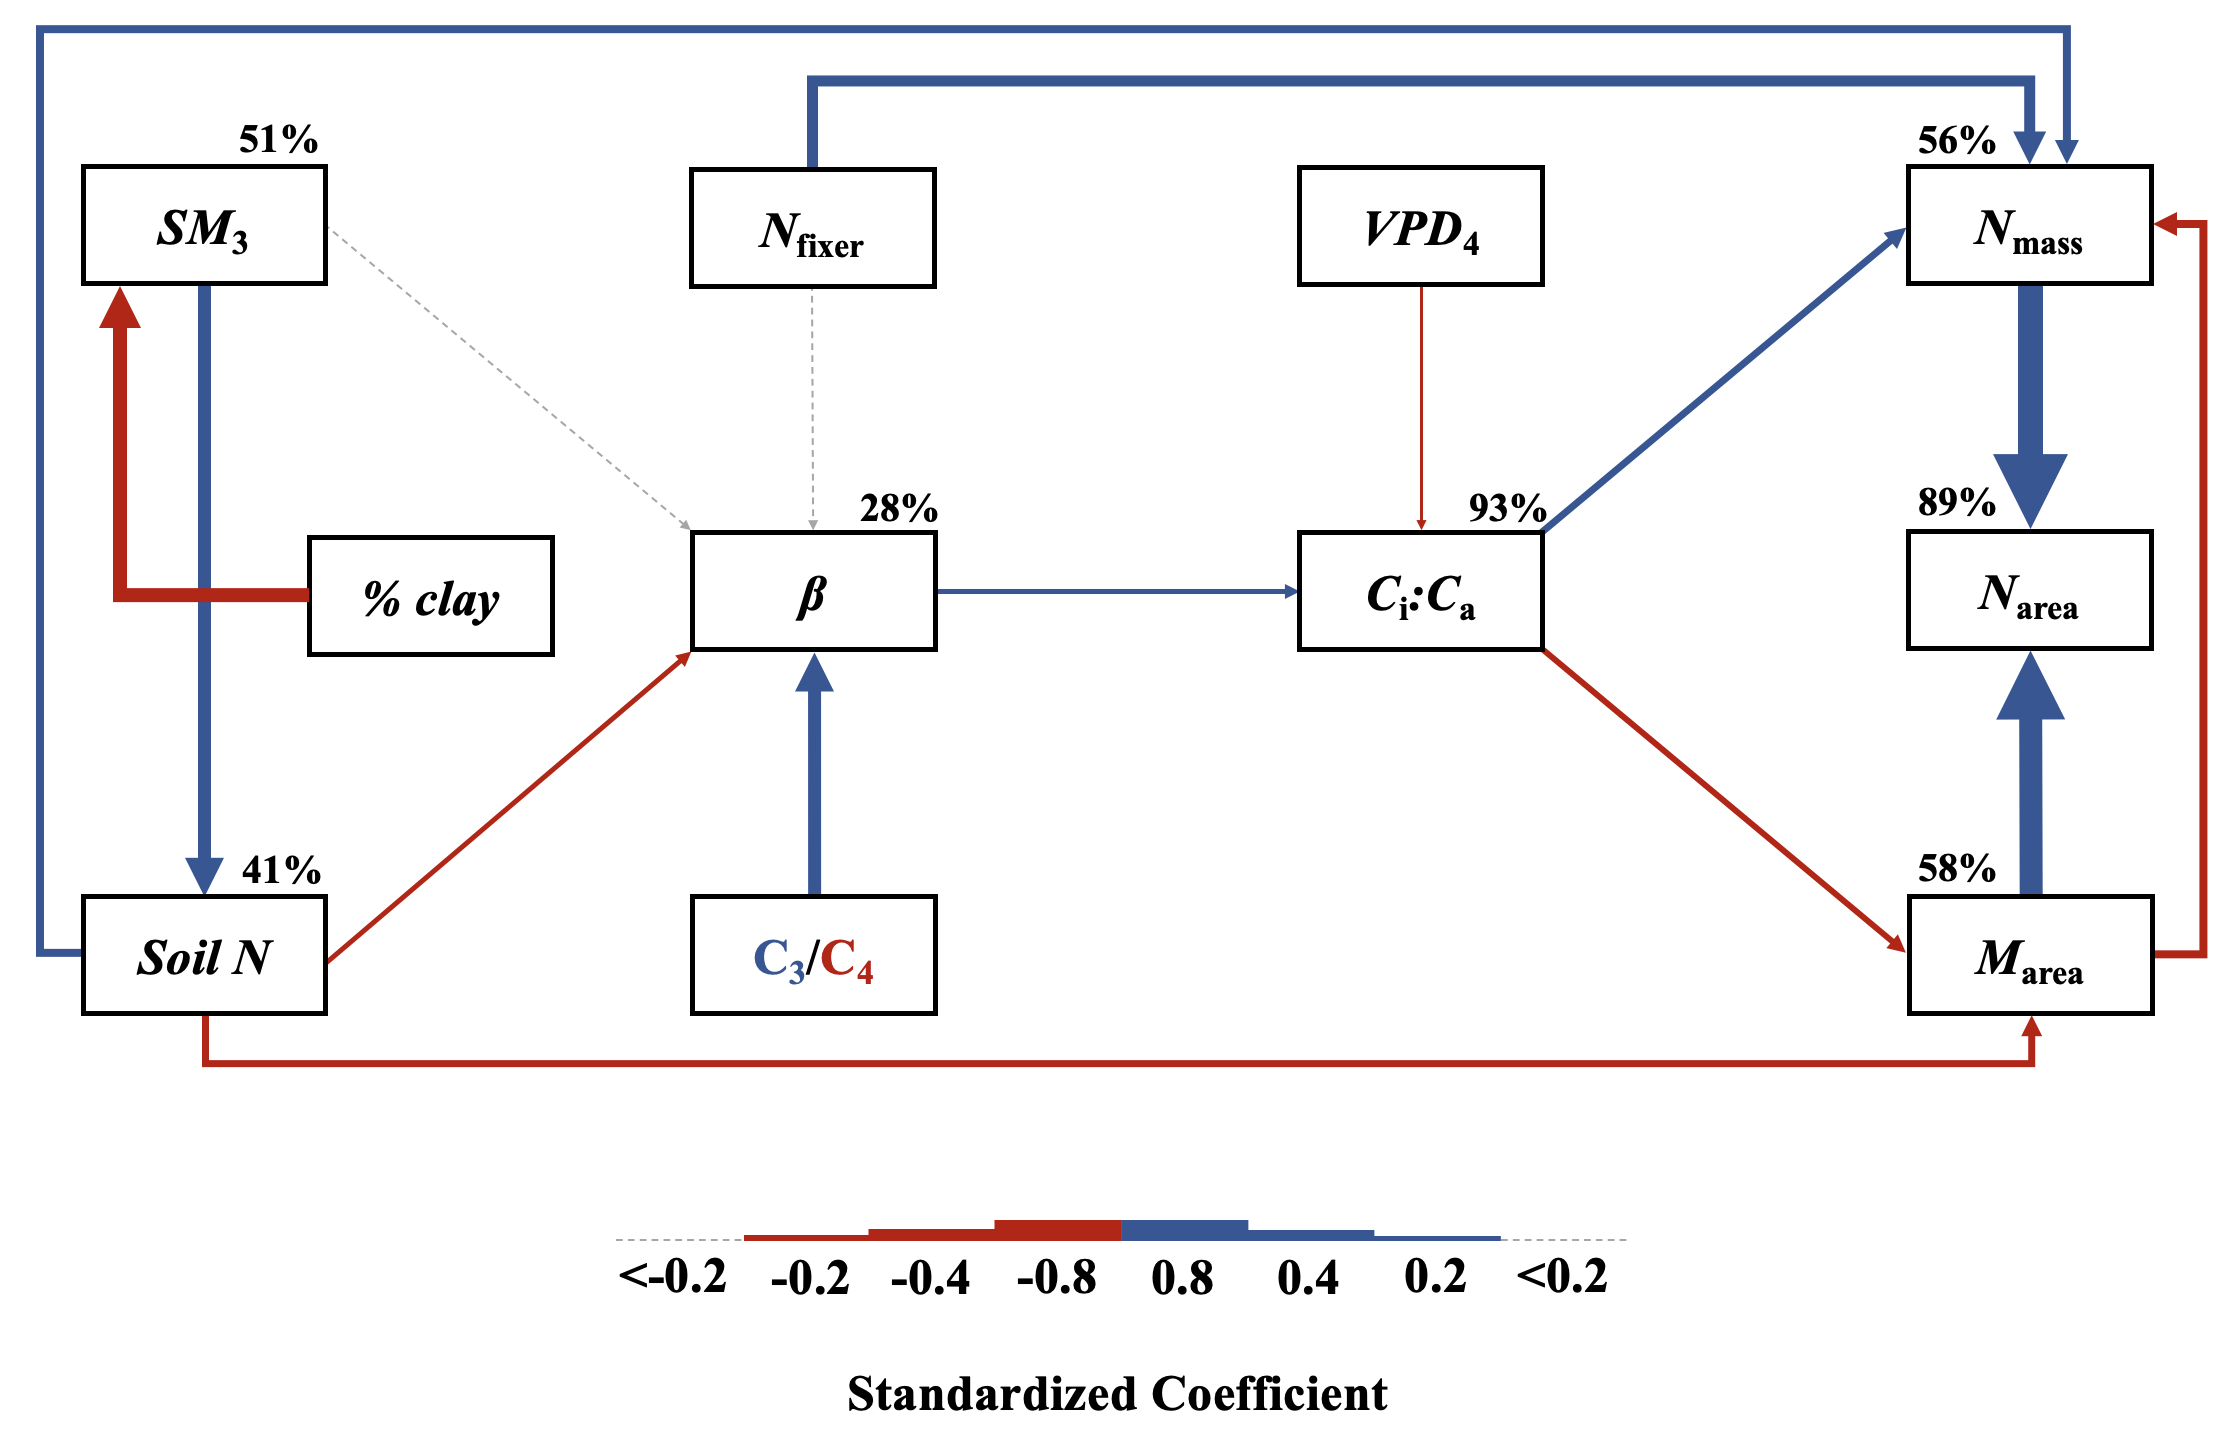
\includegraphics[width=\textwidth]{ch4_TXeco/figs/TXeco_fig5_SEM.jpg}
        \caption[Structural equation model results exploring drivers of $N_\mathrm{area}$]{Structural equation model results exploring drivers of $N_\mathrm{area}$. Boxes indicate measured edaphic factors, climatic factors, and leaf traits. Solid arrows indicate bivariate relationships where \textit{p}<0.05, while dashed arrows indicate relationships where \textit{p}>0.05. Positive model coefficients are indicated through blue arrows, negative model coefficients are indicated through red arrows, and insignificant coefficients are indicated through gray dashed arrows. Arrow thickness scales with the standardized model coefficient of each bivariate relationship. A positive coefficient for photosynthetic pathway indicates larger values in C$_3$ species, while a positive coefficient for N\textsubscript{fixer} indicates larger values in N-fixing species. Standardized model coefficients and associated \textit{p}-values are reported in Table \ref{tab:table4.5}, with conditional R$^2$ values for each response variable reported on the top right of each box.}
        \label{fig:figure4.5}
    \end{figure}
\clearpage

\section{Discussion}
\noindent In this study, direct and indirect effects of edaphic and climatic characteristics on $N_\mathrm{area}$ and components of $N_\mathrm{area}$ ($N_\mathrm{mass}$ and $M_\mathrm{area}$) were quantified in 504 individuals spanning across a soil resource availability and climate gradient in Texas, USA. Consistent patterns emerged in support of those expected from photosynthetic least-cost theory, a result driven by a strong direct negative relationship between leaf $C_\mathrm{i}$:$C_\mathrm{a}$ and $N_\mathrm{area}$ mediated through changes in $M_\mathrm{area}$. In further support of patterns expected from theory, increasing soil nitrogen availability had a negative effect on $\beta$, resulting in an indirect stimulation in $N_\mathrm{area}$ mediated through a positive relationship between $\beta$ and $C_\mathrm{i}$:$C_\mathrm{a}$. Increasing vapor pressure deficit also indirectly increased $N_\mathrm{area}$ through a direct negative effect of increasing vapor pressure deficit on leaf $C_\mathrm{i}$:$C_\mathrm{a}$, following hypotheses and patterns expected from theory. Interestingly, a positive association between soil moisture and $N_\mathrm{area}$ was driven by covariance between soil moisture and soil nitrogen availability and was not associated with a direct effect of soil moisture on $\beta$. Overall, results provide strong and consistent support for patterns expected from photosynthetic least-cost theory, showing that both soil resource availability and climate drive variance in $N_\mathrm{area}$ through changes in leaf $C_\mathrm{i}$:$C_\mathrm{a}$.

\begin{singlespace}
\subsection{\textit{Negative effects of leaf $C_\mathrm{i}$:$C_\mathrm{a}$ on $N_\mathrm{area}$ are driven by reductions in $M_\mathrm{area}$, not $N_\mathrm{mass}$}}
\end{singlespace}
\noindent The negative response of $N_\mathrm{area}$ to increasing leaf $C_\mathrm{i}$:$C_\mathrm{a}$ is consistent with previous environmental gradient \shortcite{Dong2017,Querejeta2022} and manipulation experiments (\ref{fig:figure3.4}c), showing strong support for the nitrogen-water use tradeoffs expected from photosynthetic least cost theory \shortcite{Wright2003,Prentice2014}. Negative effects of increasing leaf $C_\mathrm{i}\mathrm{:}C_\mathrm{a}$ on $N_\mathrm{area}$ were driven by  negative effect of increasing leaf $C_\mathrm{i}$:$C_\mathrm{a}$ on $M_\mathrm{area}$ coupled with a weak positive effect of increasing leaf $C_\mathrm{i}$:$C_\mathrm{a}$ on $N_\mathrm{mass}$, suggesting that changes in $N_\mathrm{area}$ across the environmental gradient were driven more strongly by changes in leaf morphology than leaf chemistry. Interestingly, the negative relationship between $M_\mathrm{area}$ and $N_\mathrm{mass}$ suggested that stimulations in $N_\mathrm{mass}$ were often associated with larger, thinner leaves (i.e., lower $M_\mathrm{area}$). These results are consistent with patterns reported from previous studies indicating that variance in $N_\mathrm{area}$ is driven by changes in $M_\mathrm{area}$ across environmental gradients, and that part of this response is due to negative covariance between $M_\mathrm{area}$ and $N_\mathrm{mass}$ \shortcite{Dong2017,Dong2020}. Negative covariance between $M_\mathrm{area}$ and $N_\mathrm{mass}$ could be a response associated with tradeoffs between leaf longevity and leaf productivity \shortcite{Wright2004,Dong2017,Dong2022a,Querejeta2022,Wang2023}.

The negative relationship between leaf $C_\mathrm{i}$:$C_\mathrm{a}$ and $M_\mathrm{area}$ could be indicative of tradeoffs between leaf longevity and leaf productivity. Tradeoffs between leaf longevity and leaf productivity are commonly observed and are included in a continuum of coordinated leaf traits that position individuals along a fast- or slow-growing leaf economics spectrum \shortcite{Wright2003,Onoda2004,Reich2014,Onoda2017,Wang2023}. Negative relationships between leaf $C_\mathrm{i}$:$C_\mathrm{a}$ and $M_\mathrm{area}$ indicate that increased stomatal conductance and reduced water use efficiency were associated with thinner, larger leaves (i.e., lower $M_\mathrm{area}$). Combined with the negative covariance between $M_\mathrm{area}$ and $N_\mathrm{mass}$ mentioned above, these responses may have allowed individuals to maximize light interception and productivity by exploiting high light environments at the expense of increased water loss and decreased water-use efficiency. This strategy may be especially advantageous for fast-growing species in open canopy systems. In this study, C$_3$ N-fixers and C$_3$ non-fixers dominated the dataset (77\% of total sampling effort), of which 23\% (17\% of total sampling effort) were classified as annual species with short growing seasons. We observed no effect of leaf $C_\mathrm{i}$:$C_\mathrm{a}$ on $N_\mathrm{area}$ or $M_\mathrm{area}$ in C$_4$ non-fixers, which made up 23\% of the sampling effort and were generally classified as warm season graminoid species with slower growth rates and longer growing seasons. These patterns indicate that stronger tradeoffs between nitrogen and water use may be more apparent in fast-growing species with high demand for building and maintaining productive leaf tissues.

\begin{singlespace}
\subsection{\textit{Soil nitrogen availability increases $N_\mathrm{area}$ through changes in $\beta$}}
\end{singlespace}
\noindent The structural equation model indicated multiple pathways where increasing soil nitrogen availability increased $N_\mathrm{area}$. First, $N_\mathrm{area}$ increased with increasing soil nitrogen availability due to larger positive direct effects of increasing soil nitrogen availability on $N_\mathrm{mass}$ than the corresponding negative direct effect of increasing soil nitrogen availability on $M_\mathrm{area}$. These patterns corroborate those observed in the individual linear mixed effect models and previous work. Second, soil nitrogen availability increased $N_\mathrm{area}$ indirectly through reductions in $\beta$, which increased leaf $C_\mathrm{i}$:$C_\mathrm{a}$ and stimulated $N_\mathrm{area}$ through a stronger negative effect of increasing leaf $C_\mathrm{i}$:$C_\mathrm{a}$ on $M_\mathrm{area}$ than corresponding positive effect of increasing leaf $C_\mathrm{i}$:$C_\mathrm{a}$ on $N_\mathrm{mass}$. Reductions in $\beta$ with increasing soil nitrogen availability were likely driven by reductions in the cost of acquiring and using nitrogen, following patterns observed in previous experiments \shortcite{Bae2015,Eastman2021,Perkowski2021,Lu2022}. These pathways indicate that soil nitrogen availability can have direct positive effects on $N_\mathrm{area}$ by increasing leaf nitrogen concentration, following previous work \shortcite{Firn2019,Liang2020},or can alternatively have indirect positive effects on $N_\mathrm{area}$ through changes in leaf morphology associated with a reduction in the cost of acquiring nitrogen, following patterns expected from photosynthetic least-cost theory. Results reported here indicate that photosynthetic least-cost frameworks are capable of detecting predictable variance in $N_\mathrm{area}$ and tradeoffs between nitrogen and water use across soil nitrogen availability gradients.

\begin{singlespace}
\subsection{\textit{Soil moisture increases $N_\mathrm{area}$ by facilitating increases in soil nitrogen availability}}
\end{singlespace}
\noindent Increasing soil moisture had a positive effect on $N_\mathrm{area}$, though this response was associated with a null effect of soil moisture on $\beta$. These results contrast patterns expected from theory, where increasing soil moisture is expected to indirectly decrease $N_\mathrm{area}$ through an increase in $\beta$ due to a reduction in costs associated with water acquisition and use \shortcite{Wright2003,Prentice2014,Lavergne2020}. Interestingly, structural equation model results revealed a strong positive association between soil moisture and soil nitrogen availability, indicating an indirect positive effect of increasing soil moisture on $N_\mathrm{area}$ mediated by the negative effect of increasing soil nitrogen availability on $\beta$. In Texan grasslands, productivity and nutrient uptake are often co-limited by precipitation and nutrient availability \shortcite{Yahdjian2011,Wang2017_NPP_stability}. Thus, increases in soil moisture may have facilitated more favorable and productive environments for soil microbial communities \shortcite{Reichman1966,Stark1995,Paul2003}, or alternatively greater nitrogen mobility in soil solution. As discussed above, the positive indirect response of $N_\mathrm{area}$ to increasing soil nitrogen availability as mediated through reductions in $\beta$ follow patterns expected from theory.

\begin{singlespace}
\subsection{\textit{Indirect effects of climate on $N_\mathrm{area}$ are mediated through changes in leaf $C_\mathrm{i}$:$C_\mathrm{a}$ and $\beta$}}
\end{singlespace}
\noindent In support of hypotheses and patterns expected from theory, increasing vapor pressure deficit indirectly increased $N_\mathrm{area}$, mediated through the negative effect of increasing vapor pressure deficit on leaf $C_\mathrm{i}$:$C_\mathrm{a}$. These responses are consistent with previous work noting strong reductions in stomatal conductance with increasing vapor pressure deficit \shortcite{Oren1999,Novick2016,Sulman2016,Grossiord2020,Lopez2021}, a response that allows plants to minimize water loss as a result of high atmospheric water demand. Results also support findings from previous experiments across environmental gradients, where increasing vapor pressure deficit generally increases $N_\mathrm{area}$ at lower stomatal conductance across environmental gradients \shortcite{Dong2017,Dong2022a,Paillassa2020,Westerband2023}. The increase in $N_\mathrm{area}$ with increasing vapor pressure deficit could allow plants to maximize photosynthetic capacity under reduced stomatal conductance \shortcite{Dong2022a}, though this pattern contrasts previous work suggesting that long-term increases in vapor pressure deficit are associated with increased plant mortality, reduced net primary productivity, and perhaps reductions in net photosynthesis rates over time due to prolonged stomatal closure \shortcite{Eamus2013,Yuan2019,Grossiord2020}. Importantly, such negative effects of increasing vapor pressure deficit often occur along much broader timescales compared to the timescale used here.  Responses observed here suggest that variance in $N_\mathrm{area}$ across environmental gradients is a deterministic acclimation response to changing aboveground climate, allowing plants to satisfy demand to build and maintain photosynthetic enzymes and optimize photosynthetic processes by maximizing resource use efficiency \shortcite{Paillassa2020,Peng2021,Dong2022a,Westerband2023}.


\begin{singlespace}
\subsection{\textit{Species identity traits modify effects of the environment on $\beta$, leaf $C_\mathrm{i}$:$C_\mathrm{a}$, and $N_\mathrm{area}$}}
\end{singlespace}
\noindent N-fixing species had greater $N_\mathrm{area}$ values on average compared to non-fixing sp-ecies, a pattern driven by a stronger stimulation in $N_\mathrm{mass}$ in N-fixing species coupled with no change in $M_\mathrm{area}$ between species with different N-fixation ability. There was no evidence to suggest that N-fixing species had different $\beta$ or leaf $C_\mathrm{i}$:$C_\mathrm{a}$ values compared to non-fixing species across the environmental gradient. These results follow patterns from previous environmental gradient experiments that investigate variance in leaf nitrogen allocation in N-fixing species \shortcite{Adams2016,Dong2017,Dong2020}, and that increases in $N_\mathrm{mass}$ and $N_\mathrm{area}$ in N-fixing species are not necessarily correlated to increases in water use efficiency or reductions in leaf $C_\mathrm{i}$:$C_\mathrm{a}$ \shortcite{Adams2016}. While results are consistent with results from previous environmental gradient experiments, they do not support hypotheses presented here or patterns expected form theory, which predicts that stimulations in $N_\mathrm{area}$ by N-fixing species should be driven by a reduction in $\beta$ relative to non-fixing species, and that this response should decrease stomatal conductance and leaf $C_\mathrm{i}$:$C_\mathrm{a}$.
    
C$_4$ species had reduced $\beta$, leaf $C_\mathrm{i}$:$C_\mathrm{a}$, and $N_\mathrm{area}$ than C$_3$ species. Reduced $\beta$ and leaf $C_\mathrm{i}$:$C_\mathrm{a}$ values in C$_4$ species follow hypotheses listed above, a pattern that could be the result of either reduced costs of nitrogen acquisition and use, increased costs of water acquisition and use, or both \shortcite{Wright2003,Prentice2014}. Results also indicate that $\beta$ in C$_4$ non-fixers was unresponsive to changes in soil nitrogen availability despite an apparent negative effect of increasing soil nitrogen availability on $\beta$ in C$_3$ N-fixers and C$_3$ non-fixers. Combined with a general null response of $\beta$ to soil moisture regardless of plant functional group, these patterns imply that reduced $\beta$ values in C$_4$ species may be the result of lower costs of nitrogen acquisition and use relative to C$_3$ species. While lower $\beta$ values in C$_4$ species provides a possible explanation for why C$_4$ species often have lower leaf $C_\mathrm{i}$:$C_\mathrm{a}$ and greater water use efficiency, theory predicts that this response should cause C$_4$ species to have greater $N_\mathrm{area}$ values compared to C$_3$ species, though C$_4$ species commonly exhibit lower $N_\mathrm{area}$ and higher nitrogen use efficiency than C$_3$ species \shortcite{Schmitt1981,Sage1987_c3c4,Ghannoum2011}. We speculate that lowered costs of nitrogen acquisition and use in C$_4$ species could be driven by more efficient Rubisco carboxylation efficiency in C$_4$ species associated with CO$_2$ concentrating mechanisms that eliminate photorespiration \shortcite{Ghannoum2011}, which could reduce or eliminate the need to sacrifice inefficient nitrogen use for efficient water use to achieve optimal photosynthesis rates.

\subsection{\textit{Next steps for optimality model development}}
\noindent Optimality models for both C$_3$ and C$_4$ species have been developed using principles from photosynthetic least-cost theory \shortcite{Prentice2014,Wang2017,Smith2019,Stocker2020,Scott2022}. In both C$_3$ and C$_4$ model variants, $\beta$ values are held constant using global datasets of leaf $\delta^{13}$C \shortcite{Wang2017,Cornwell2018}. Specifically, the C$_3$ optimality model initially assumed a constant $\beta$ value of 240 \shortcite{Wang2017}, later corrected to 146 \shortcite{Stocker2020}, while the C$_4$ optimality model assumes a constant $\beta$ value of 166 \shortcite{Scott2022}. These results, which build on findings from \shortciteN{Paillassa2020} and \shortciteN{Lavergne2020}, demonstrate high variability in calculated $\beta$ values across the environmental gradient. Specifically, $\beta$ values in C$_3$ species ranged from 1.7 to 188.0 (mean: 30.2; median: 23.1; standard deviation: 25.4), while ranged from 0.1 to 110.6 in C$_4$ species (mean: 7.2; median: 0.7; standard deviation: 18.6). Mean $\beta$ values in both C$_3$ and C$_4$ species were consistently lower than values currently implemented in optimality models, though this was likely the result of increased water limitation across sites relative to global averages. Regardless, the high degree of $\beta$ variability across this environmental gradient, together with findings from \shortciteN{Lavergne2020} and \shortciteN{Paillassa2020}, suggests that the use of constant $\beta$ values may contribute to erroneous errors when conducting optimality model simulations. Results from this experiment build on suggestions from \shortciteN{Wang2017}, suggesting that future photosynthetic least-cost optimality model developments should consider adopting frameworks for dynamically calculating $\beta$.

\subsection{\textit{Conclusions}}
\noindent To summarize, variability in $N_\mathrm{area}$ across an environmental gradient in Texan grasslands was driven by indirect effects of climate and soil resource availability mediated by changes in $\beta$ and leaf $C_\mathrm{i}$:$C_\mathrm{a}$. Results from this experiment provide strong and consistent support for patterns expected from photosynthetic least-cost theory, demonstrating that negative relationships between $C_\mathrm{i}$:$C_\mathrm{a}$ and $N_\mathrm{area}$ unify expected effects of climatic and edaphic characteristics on $N_\mathrm{area}$ across environmental gradients. Results reported here also demonstrate a need to consider the dynamic nature of the relative cost of nitrogen versus water uptake ($\beta$) across environmental gradients in optimality models that leverage principles of photosynthetic least-cost theory.
